%% 
%% Copyright 2019-2024 Elsevier Ltd
%% 
%% Elsevier CAS LaTeX Single-Column Research Manuscript
%% 
\documentclass[a4paper,fleqn]{cas-sc}

\usepackage[authoryear,longnamesfirst]{natbib}
\usepackage{amsmath,amssymb,amsfonts}
\usepackage{graphicx}
\usepackage{booktabs}
\usepackage{array}
\usepackage{multirow}
\usepackage{tabularx}
\usepackage{dcolumn}
\usepackage{microtype}

%%% Author macros
\def\tsc#1{\csdef{#1}{\textsc{\lowercase{#1}}\xspace}}
\tsc{WGM}
\tsc{QE}

\begin{document}
\let\WriteBookmarks\relax
\def\floatpagepagefraction{1}
\def\textpagefraction{.001}

% Short title and authors
\shorttitle{AI-Driven Spatiotemporal Modeling of Urban Heat Island Dynamics in Mumbai}
\shortauthors{A. Ansari et~al.}

% Main title of the paper
\title [mode = title]{AI-Driven Spatiotemporal Modeling and Downscaling of Urban Heat Island Dynamics in Metropolitan Mumbai}

% Author metadata
\author[1]{Abdulrehman Ansari}[orcid=0000-0002-8921-4321]
\cormark[1]
\ead{abdulrehman.ansari@student.mhssce.ac.in}
\credit{Conceptualization, Cloud Architecture, Geospatial Dashboard, Writing - original draft}

\author[1]{Mohd Hussain Siddique}[orcid=0000-0001-7643-9182]
\credit{System Architecture, Remote Sensing Extraction, ML Downscaling Regressor, Simulation Engine}

\author[1]{Asad Shaikh}[orcid=0000-0003-1289-5430]
\credit{Data Engineering, Meteorological Ingestion, Spatial Block Cross-Validation, Explainable AI}

\author[1]{Shah Mohd Ahmad}[orcid=0000-0002-4519-7801]
\credit{Quality Assurance, Statistical Validation, Pipeline Testing, Manuscript Review \& Editing}

% Affiliation
\affiliation[1]{organization={Department of Computer Engineering, M.H. Saboo Siddik College of Engineering, Affiliated to University of Mumbai},
            addressline={8, Saboo Siddik Polytechnic Road, Byculla}, 
            city={Mumbai},
            postcode={400008}, 
            state={Maharashtra},
            country={India}}

\cortext[1]{Corresponding author}

% Abstract
\begin{abstract}
Urban Heat Island (UHI) effects pose severe environmental and public health hazards in rapidly expanding coastal megacities, where dense built-up fabrics, loss of vegetative canopies, high ambient humidity, and maritime boundary layer interactions generate complex thermal regimes. Satellite thermal infrared remote sensing provides spatial coverage of Land Surface Temperature (LST), yet sensors face an inherent trade-off between spatial and temporal resolutions. Furthermore, conventional machine learning downscaling models frequently employ random train--test partitioning, which violates Tobler's First Law of Geography and introduces substantial spatial autocorrelation leakage, producing artificially optimistic validation scores that fail to generalize across non-contiguous municipal districts. In this study, an AI-driven spatiotemporal modeling and downscaling framework is established for Metropolitan Mumbai ($437.71\text{ km}^2$, 24 municipal wards of the Brihanmumbai Municipal Corporation). The architecture ingests multi-source satellite observations from Landsat 8/9 Level-2, Sentinel-2, and SRTM digital elevation data alongside a 28-year continuous ground meteorological archive from the India Meteorological Department (IMD) comprising 383,640 hourly observations (1997--2024). Atmospheric time series undergo automated quality filtering via rolling Hampel $3\sigma$ Median Absolute Deviation outlier rejection, physical bounds enforcement, monotonic PCHIP spline gap filling, orthogonal wind velocity decomposition ($u, v$), and vapor pressure deficit (VPD) computation before synchronizing with the $\sim$10:00--11:30~IST satellite overpass. A unified 17-dimensional biophysical and atmospheric predictor matrix is constructed to drive gradient-boosted decision trees (XGBoost) and Random Forest ensembles. Spatially independent validation via SpatialBlockKFold with an empirical 1.2~km exclusion buffer based on Moran's $I$ semivariogram range demonstrates robust generalization ($\text{RMSE} = 0.835^\circ\text{C}$, $R^2 = 0.826$, $\text{MAE} = 0.675^\circ\text{C}$ for IMD-enriched XGBoost), while revealing that naive random partitioning underestimates true spatial error by over $0.54^\circ\text{C}$. Non-parametric Mann--Kendall and Sen's slope analyses prove a statistically significant multi-decadal warming trend of $+0.044^\circ\text{C}/\text{year}$ ($+0.44^\circ\text{C}/\text{decade}$, $p = 3.64 \times 10^{-5}$, $Z = +4.129$). TreeSHAP game-theoretic attribution decomposes microclimatic drivers, identifying impervious built-up density (NDBI) as the dominant warming agent ($+1.41^\circ\text{C}$), while vegetation canopy (NDVI, $-0.42^\circ\text{C}$), surface albedo ($-0.38^\circ\text{C}$), and coastal proximity ($-0.36^\circ\text{C}$) supply vital cooling moderation. Finally, a high-speed simulation engine assesses localized urban cooling interventions, demonstrating that aggressive greening and cool-roof deployment can alleviate localized surface temperatures by up to $-0.94^\circ\text{C}$, yielding annual cooling energy savings of $4.50\text{ kWh/m}^2/\text{year}$ with sub-5~ms computational inference latency. The integrated framework establishes an empirical, reproducible foundation for evidence-based thermal mitigation in dense coastal environments across the Global South.
\end{abstract}

% Highlights
\begin{highlights}
\item Developed an AI spatiotemporal framework fusing multi-source remote sensing with 28-year (383,640 records) quality-controlled meteorological data for Mumbai.
\item Reconstructed 30~m Land Surface Temperature using gradient-boosted decision trees on a unified 17-dimensional biophysical predictor space.
\item Implemented Spatial Block cross-validation with a 1.2~km buffer exclusion zone to eliminate spatial autocorrelation data leakage.
\item Confirmed statistically significant multi-decadal urban warming of $+0.44^\circ\text{C}$ per decade ($p = 3.64 \times 10^{-5}$) using Mann--Kendall and Sen's tests.
\item Quantified marginal biophysical thermal drivers using TreeSHAP and demonstrated interactive cooling intervention simulations saving up to $4.50\text{ kWh/m}^2/\text{year}$.
\end{highlights}

% Keywords
\begin{keywords}
Urban Heat Island \sep Land Surface Temperature \sep Machine Learning \sep Spatiotemporal Downscaling \sep Spatial Block Cross-Validation \sep Explainable Artificial Intelligence \sep TreeSHAP \sep Urban Heat Mitigation
\end{keywords}

\maketitle

\section{Introduction}
\label{sec:introduction}

The Urban Heat Island (UHI) phenomenon represents one of the most visible and consequential environmental manifestations of rapid global urbanization. As natural permeable surfaces, vegetative canopies, and water bodies are systematically replaced by high-density impervious surfaces such as asphalt, concrete, and masonry, the surface radiation budget and turbulent sensible heat fluxes undergo profound alterations. Impervious construction materials exhibit high solar absorptivity, low surface albedo, and substantial thermal inertia, allowing them to absorb incoming shortwave solar radiation during daylight hours and release it as longwave thermal radiation well into the nocturnal boundary layer. Concurrently, the reduction in vegetated cover suppresses latent heat loss through evapotranspiration, thereby concentrating the surface energy balance into elevated sensible heat flux. The resulting elevated thermal footprint directly elevates Land Surface Temperature (LST) and ambient air temperature across urban agglomerations, compounding urban heat stress, deteriorating ambient air quality through photochemical ozone formation, elevating heat-related morbidity and mortality, and driving peak electricity demand for building cooling systems.

The challenges imposed by urban thermal intensification are exceptionally acute in tropical and subtropical coastal megacities, among which Metropolitan Mumbai represents an exemplary and critical case study. Located along the west coast of India, Mumbai exhibits extreme demographic density (exceeding 20,000~persons/km$^2$ across multiple municipal wards), hyper-dense built infrastructure, widespread informal settlements with uninsulated corrugated sheet roofing, and rapid ongoing land reclamation. The city's geography is fundamentally shaped by its peninsular configuration, bounded by the Arabian Sea to the west and south, and Thane Creek to the east. This maritime setting introduces complex mesoscale coastal atmospheric interactions, including sea-breeze circulations, maritime thermal buffering, and persistently high relative humidity. Under conditions of elevated ambient humidity, the human body's evaporative cooling efficiency through perspiration is severely curtailed, dramatically escalating the wet-bulb globe temperature and magnifying human physiological heat stress far beyond what dry-bulb temperature measurements indicate alone.

Accurate spatial and temporal quantification of urban heat dynamics is indispensable for evidence-based urban resilience planning and targeted municipal mitigation. Satellite thermal infrared (TIR) remote sensing has traditionally served as the primary instrument for characterizing spatial LST distributions. However, Earth observation satellite systems are constrained by an inherent physical trade-off between spatial and temporal resolutions. Sensors that provide high spatial resolution, such as the Thermal Infrared Sensor (TIRS/TIRS-2) onboard Landsat~8 and Landsat~9, deliver thermal radiometry at 100~m spatial resolution (resampled by the United States Geological Survey to 30~m), but possess a 16-day orbital revisit cycle that is frequently disrupted by persistent cloud cover during the pre-monsoon and monsoon periods. Conversely, high-temporal-revisit instruments, such as the Moderate Resolution Imaging Spectroradiometer (MODIS) onboard the Terra and Aqua platforms or the Visible Infrared Imaging Radiometer Suite (VIIRS), provide daily observations but at coarse spatial resolutions of 375~m to 1~km, which completely obscure localized neighborhood-scale thermal variations, street-canyon microclimates, and informal settlement hot spots. Ground meteorological stations operated by national agencies, such as the India Meteorological Department (IMD), provide continuous high-frequency temporal observations, yet their spatial density is exceptionally sparse, with only two principal synoptic ground stations (Colaba in South Mumbai and Santacruz in the western suburbs) serving an administrative expanse exceeding 437~km$^2$.

To overcome this resolution dilemma, thermal downscaling techniques have emerged as a prominent area of research, seeking to sharpen coarse-resolution thermal observations to neighborhood-scale resolutions by establishing statistical or empirical relationships with finer-scale auxiliary predictors, such as multispectral vegetation and built-up indices, surface albedo, and digital elevation models. In recent years, machine learning algorithms, particularly nonlinear tree-based ensembles such as Random Forest and gradient-boosted decision trees (e.g., XGBoost), have demonstrated marked superiority over traditional linear regression and bicubic interpolation approaches. These algorithms possess the capacity to model complex, highly nonlinear interactions among heterogeneous surface characteristics, topography, and atmospheric variables without requiring rigid physical assumptions.

Nevertheless, existing machine learning-based LST downscaling studies suffer from four fundamental methodological limitations:
\begin{enumerate}[1.]
    \item \textbf{Disconnection from Dynamic Atmospheric Records:} Most thermal remote sensing studies rely solely on static spatial covariates derived from satellite imagery, treating thermal snapshots as isolated events without integrating multi-decadal, high-frequency in-situ meteorological records that capture ambient temperature, humidity, wind circulation vectors, and atmospheric evaporative demand.
    \item \textbf{Spatial Autocorrelation Data Leakage:} Machine learning models in environmental remote sensing are overwhelmingly evaluated using conventional random $k$-fold cross-validation or random holdout train--test splits. In spatial datasets, neighboring observations exhibit strong spatial autocorrelation, as formalized by Tobler's First Law of Geography (``everything is related to everything else, but near things are more related than distant things''). Random splitting places geographically proximate pixels simultaneously into training and validation sets, allowing the model to memorize spatial coordinates and local autocorrelations rather than learning generalized biophysical relationships. Consequently, published validation metrics (such as $R^2$ and RMSE) are heavily optimistic and degrade substantially when the models are evaluated across non-contiguous or unseen urban districts.
    \item \textbf{The Black-Box Interpretability Barrier:} While tree-based ensemble models achieve superior predictive accuracy, their internal decision logic is opaque. Conventional feature importance metrics (e.g., Gini impurity decrease or split frequency) do not indicate the directionality of feature impacts or quantify marginal temperature contributions in physical degrees Celsius. Without game-theoretic explainability, urban planners cannot discern whether a predicted hotspot is driven by impervious surface expansion, vegetative loss, or macro-geographic distance from the sea breeze.
    \item \textbf{Absence of Real-Time Policy Decision Simulators:} Existing numerical microclimate and computational fluid dynamics (CFD) simulation tools, such as ENVI-met or the Weather Research and Forecasting model coupled to Urban Canopy Models (WRF-UCM), demand prohibitive computational time (often requiring hours to days for a single neighborhood), rendering interactive scenario planning, participatory zoning analysis, and real-time municipal mitigation evaluation impossible for urban administrators.
\end{enumerate}

To rigorously address these interconnected gaps, this study presents a comprehensive, AI-driven spatiotemporal modeling and downscaling framework tailored specifically to Metropolitan Mumbai. The framework ingests and synchronizes multi-source satellite data from Google Earth Engine (Landsat~8/9 Level-2, Sentinel-2, and SRTM DEM) with a 28-year continuous ground meteorological archive from the India Meteorological Department comprising 383,640 hourly observations (1997--2024). The meteorological observations undergo automated quality filtering via Hampel Median Absolute Deviation (MAD) outlier detection, physical bounds checking, monotonic PCHIP spline imputation, orthogonal wind decomposition, and vapor pressure deficit derivation before synchronizing with the satellite overpass window. A unified 17-dimensional biophysical and atmospheric predictor matrix is constructed to drive XGBoost and Random Forest downscaling models. To enforce spatial independence, models are evaluated using SpatialBlockKFold cross-validation with an empirical 1.2~km exclusion buffer derived from the semivariogram range of Moran's $I$, preventing spatial information leakage. The trained models are subsequently decoded using TreeSHAP to quantify the exact marginal contribution of each biophysical driver, coupled with long-term Mann--Kendall and Sen's slope trend analyses, and embedded into a sub-5~ms What-If simulation engine to evaluate localized urban cooling scenarios.

The explicit objectives of this research are:
\begin{enumerate}[(i)]
    \item To construct a quality-controlled, multi-source spatiotemporal feature repository combining 30~m satellite-derived biophysical parameters with 28 years of synchronized meteorological observations across Metropolitan Mumbai.
    \item To model and downscale LST using tree-based machine learning ensembles and rigorously evaluate their spatial generalizability against conventional random holdouts using a 1.2~km spatially buffered cross-validation protocol.
    \item To decompose and attribute the biophysical and atmospheric drivers of urban thermal variance using game-theoretic TreeSHAP explainability.
    \item To quantify multi-decadal historical temperature trajectories using non-parametric Mann--Kendall and Sen's slope estimators.
    \item To execute high-speed scenario-based simulations evaluating the thermodynamic cooling efficacy and projected HVAC electrical energy savings of urban greening, cool roofs, and urban parks across Mumbai's municipal wards.
\end{enumerate}

\section{Study Area}
\label{sec:study_area}

The geographic domain of this investigation encompasses the entire official administrative jurisdiction of Metropolitan Mumbai, Maharashtra, India, administered by the Brihanmumbai Municipal Corporation (BMC). The study area spans the 24 official municipal administrative wards (designated Wards A through T) and covers a verified territorial expanse of $437.71\text{ km}^2$. The spatial domain is bounded by geographic coordinates:
\begin{equation}
    \text{Longitude: } [72.7753^\circ\text{E},\ 73.0024^\circ\text{E}], \quad \text{Latitude: } [18.8928^\circ\text{N},\ 19.2801^\circ\text{N}]
    \label{eq:bounding_box}
\end{equation}
All geospatial datasets and spatial coordinates in this study are projected onto the Universal Transverse Mercator (UTM) Zone 43 North coordinate reference system based on the WGS~84 datum (EPSG:32643), ensuring metric distance fidelity for buffer operations and spatial statistical modeling.

\begin{figure}
    \centering
    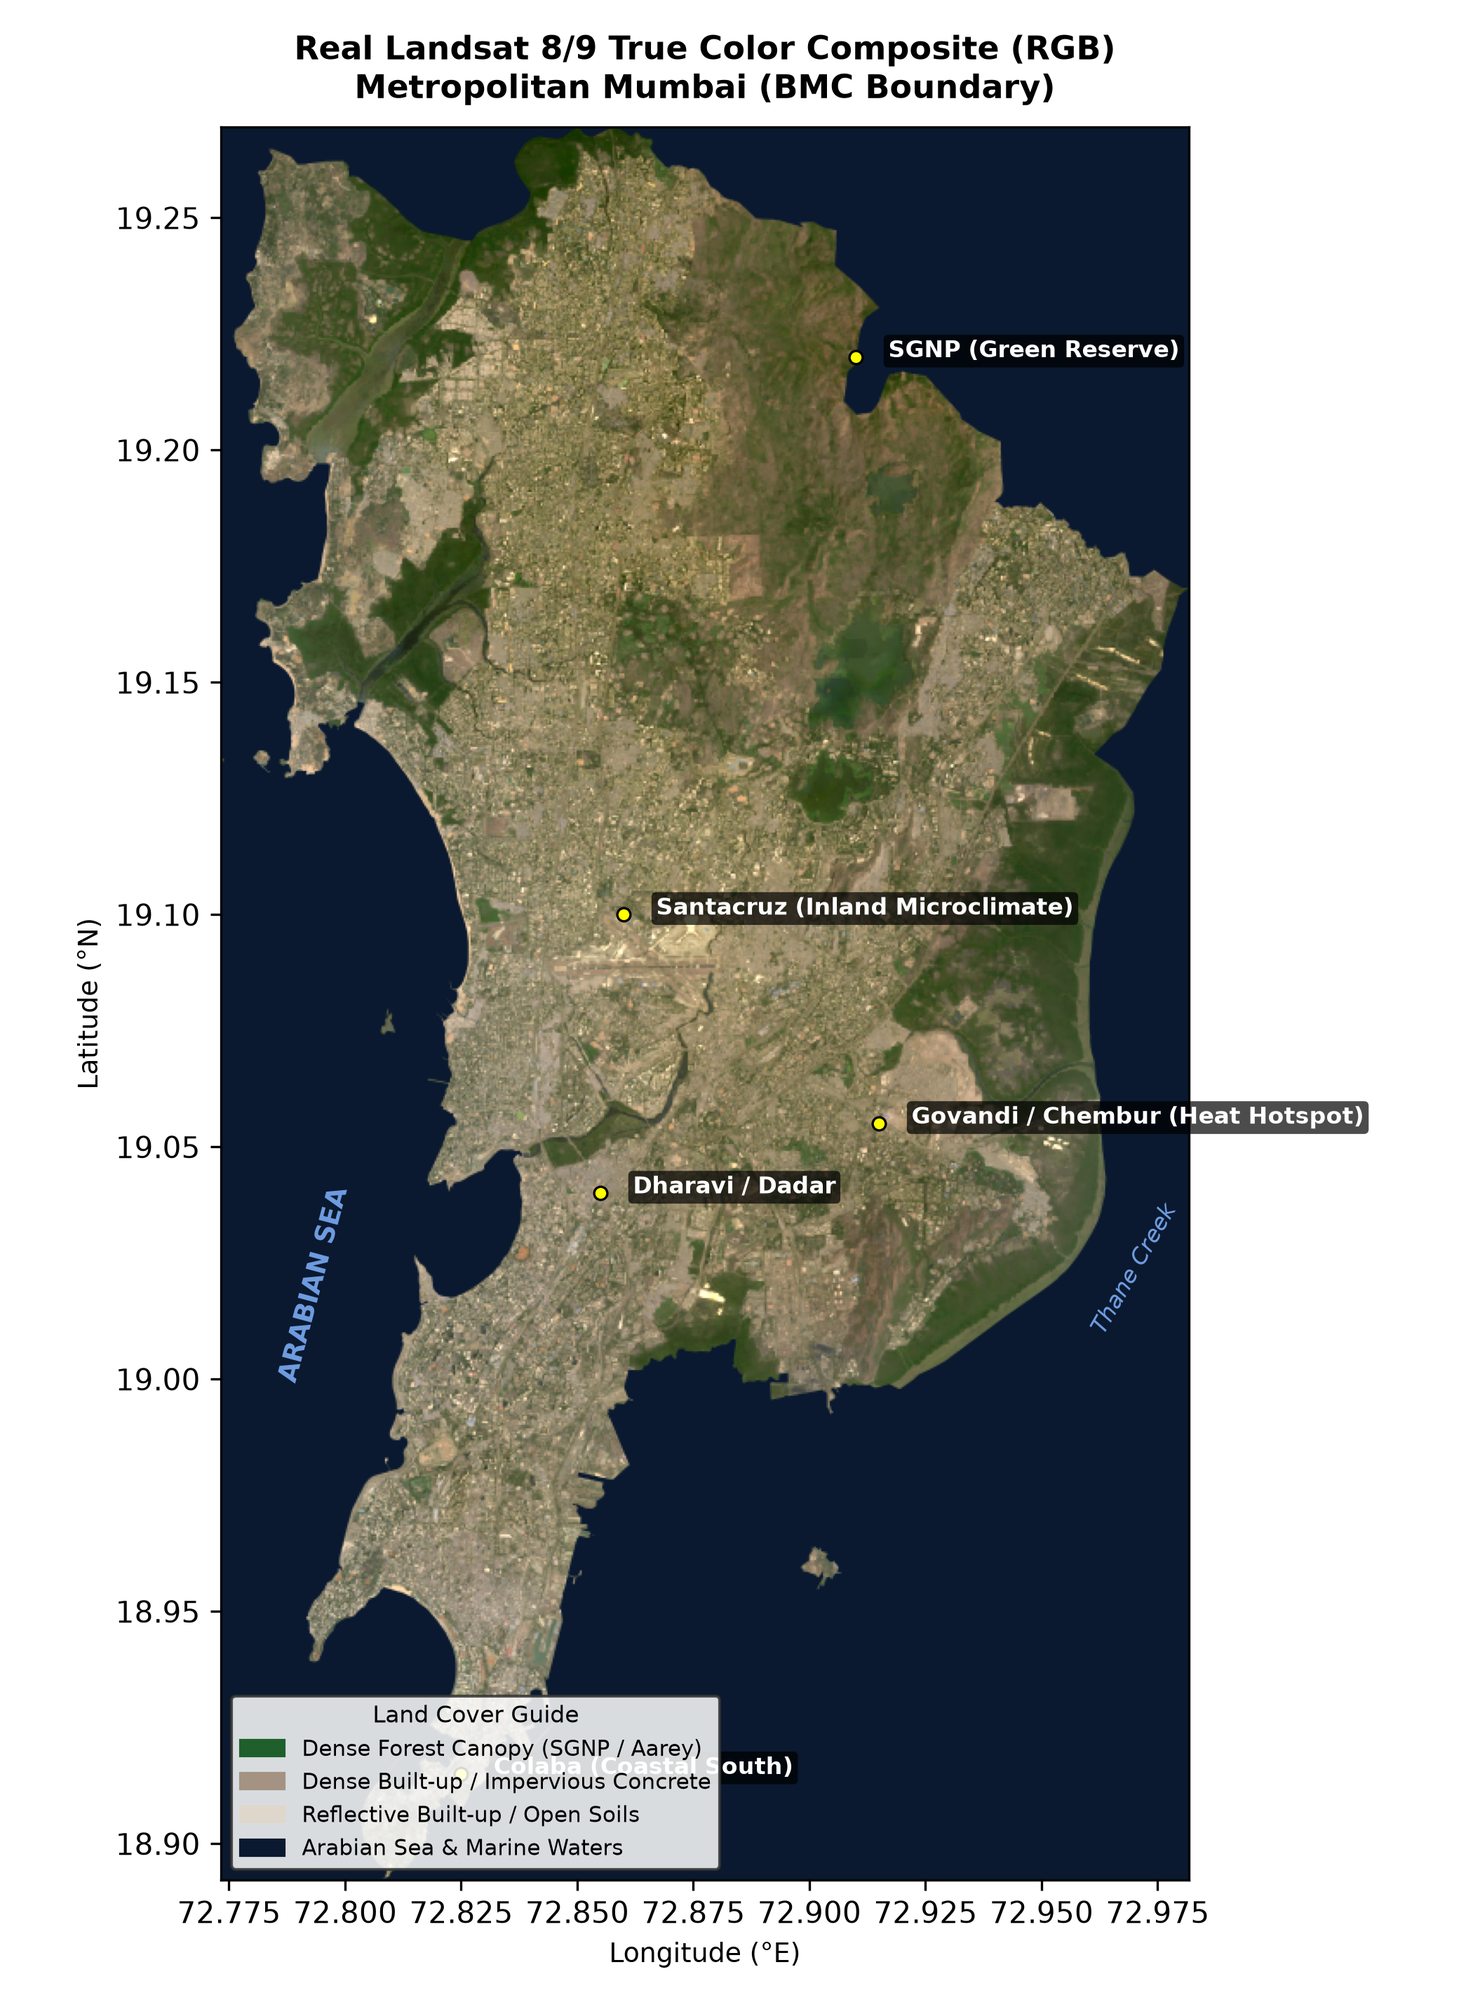
\includegraphics[width=0.72\columnwidth]{figs/review1_true_color.png}
    \caption{Geographic extent and spatial setting of Metropolitan Mumbai showing the official Brihanmumbai Municipal Corporation (BMC) administrative boundary ($437.71\text{ km}^2$), the coastal peninsula, Arabian Sea interface, Thane Creek, and the northern ecological reserve of Sanjay Gandhi National Park.}
    \label{fig:study_area}
\end{figure}

Metropolitan Mumbai represents a highly heterogeneous, tropical coastal megacity exhibiting profound morphological and microclimatic contrasts over short geographic distances. Geographically, Mumbai occupies a narrow peninsula extending southward into the Arabian Sea. It is bordered by the open Arabian Sea along its western and southern flanks, while Thane Creek and Mumbai Harbour separate the city from the mainland of Maharashtra to the east. The northern sector of the municipal territory is anchored by the Sanjay Gandhi National Park (SGNP), an expansive tropical moist deciduous ecological reserve exhibiting elevations reaching 436~m above sea level, providing an essential regional natural cooling sink and vegetative buffer.

The urban morphology of Mumbai is characterized by extreme spatial heterogeneity. Highly developed commercial business districts featuring glass-and-steel high-rises (such as the Bandra-Kurla Complex and Nariman Point) stand in stark proximity to ultra-dense, low-rise informal settlements (most notably Dharavi in Ward G/N and Govandi/Mankhurd in Ward M/E), where building densities exceed 80\% ground coverage with predominant corrugated iron and asbestos sheet roofing materials. These informal settlement fabrics exhibit negligible vegetation cover, low surface reflectivity, and restricted ventilation, generating intense local surface heat anomalies. Along the eastern and western shorelines, extensive mangrove wetlands, mudflats, and salt pans form delicate coastal ecologies that interact dynamically with the incoming marine boundary layer.

Climatically, Mumbai is classified under the Koppen-Geiger climate classification as having a tropical wet and dry climate (Aw), characterized by distinct pre-monsoon, monsoon, post-monsoon, and winter seasons. The pre-monsoon period (extending from March through May) is defined by severe thermal discomfort, characterized by intense solar insolation, elevated ambient temperatures exceeding $35^\circ\text{C}$, and high relative humidity ($60\%\text{--}85\%$) driven by persistent marine advection from the Arabian Sea. The diurnal sea-breeze circulation acts as a dynamic cooling mechanism for coastal wards (such as Colaba in Ward A), whereas inland eastern suburbs (such as Chembur and Mankhurd) experience delayed sea-breeze penetration and diminished nocturnal ventilation, leading to acute heat retention. This intricate interplay between dense urban development, maritime proximity, complex coastal topography, and socio-spatial vulnerability renders Mumbai an ideal and urgent laboratory for advanced spatiotemporal urban heat island downscaling and mitigation modeling. Figure~\ref{fig:study_area} depicts the geographic setting, coastal perimeter, and municipal extent of the study domain.

\section{Methods}
\label{sec:methods}

\subsection{Overall Methodological Framework}
\label{subsec:framework}

The research architecture developed in this study unifies remote sensing data ingestion, multi-decadal meteorological time series preprocessing, physics-based radiometric calibrations, machine learning downscaling, spatially independent validation, game-theoretic model interpretability, statistical trend analysis, and policy scenario simulation into an end-to-end analytical workflow. As illustrated in Figure~\ref{fig:methodology}, the operational framework comprises two parallel data streams:

\begin{figure}
    \centering
    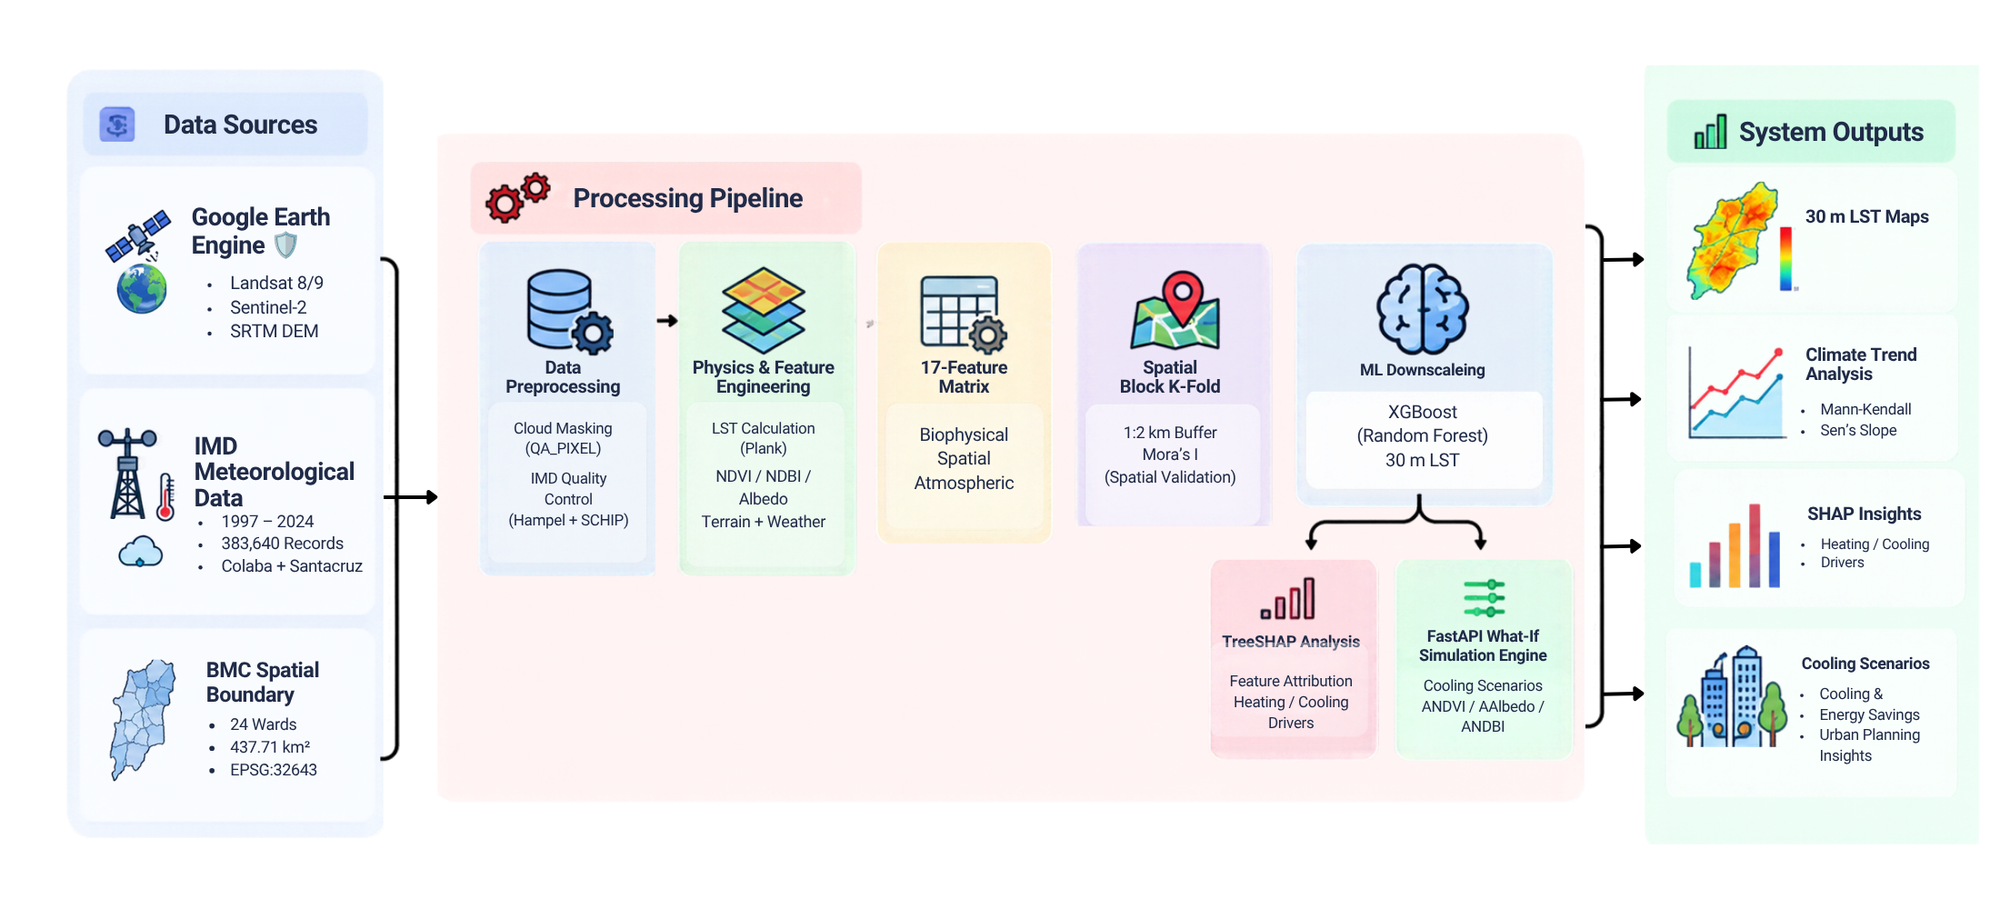
\includegraphics[width=\columnwidth]{figs/ArchitectureDiagram.png}
    \caption{End-to-end technical architecture and workflow of the Mumbai UHI Platform, showing the parallel ingestion of Google Earth Engine satellite imagery and 28-year IMD meteorological records, radiometric physics calibration, 17-dimensional predictor matrix assembly, spatial block validation with 1.2~km buffer isolation, TreeSHAP explainability, and the sub-5~ms What-If policy simulation engine.}
    \label{fig:methodology}
\end{figure}

\begin{enumerate}[1.]
    \item \textbf{Satellite Remote Sensing Stream:} Multispectral and thermal infrared imagery from Landsat~8 and Landsat~9 Collection~2 Level-2, optical bands from Sentinel-2 MSI, and elevation products from the NASA SRTM 30~m DEM are ingested programmatically via the Google Earth Engine (GEE) cloud platform. Radiometric calibration, cloud masking via pixel quality bitmasks, calculation of spectral indices (NDVI, NDBI, MNDWI), broadband surface albedo derivation, and radiative transfer modeling of LST using the Planck split-window formulation are executed across the BMC territory.
    \item \textbf{In-Situ Climatological Stream:} A continuous 28-year hourly surface weather archive (1997--2024, 383,640 records) obtained from the India Meteorological Department (IMD) is subjected to automated multi-stage quality control, including Hampel Median Absolute Deviation outlier rejection, physical bounds clipping, monotonic PCHIP spline interpolation for short missing sequences, orthogonal wind vector decomposition ($u, v$), and vapor pressure deficit (VPD) computation.
\end{enumerate}

The meteorological parameters corresponding to the Landsat orbital overpass window (10:00--11:30~IST) are extracted and merged with the satellite observations to construct a unified 17-dimensional biophysical and atmospheric predictor matrix. This predictor space drives two tree-based ensemble downscaling models: gradient-boosted decision trees (XGBoost) and Random Forest regressors. To rigorously assess spatial generalizability and eliminate spatial autocorrelation bias, a Spatial Block K-Fold validation protocol is enforced with an empirical 1.2~km buffer exclusion zone based on Moran's $I$ semivariogram range. Model predictions are interpreted using TreeSHAP to quantify marginal feature contributions in degrees Celsius. In parallel, the 28-year meteorological record is interrogated via the non-parametric Mann--Kendall test and Sen's slope estimator to establish multi-decadal urban warming trends. Finally, the trained XGBoost surrogate model is embedded within an ultra-low-latency simulation engine to evaluate localized urban greening, cool roof, and park development scenarios.

\subsection{Satellite Data Acquisition and Processing}
\label{subsec:satellite_data}

Satellite data acquisition was performed programmatically using the Google Earth Engine cloud computing environment under cloud project \texttt{uhi-mumbai-507613}. The analysis focused on the critical pre-monsoon summer season from 1~February to 31~May 2024, representing the period of maximal thermal stress and urban heat intensity in western India prior to the onset of the southwest monsoon.

A total of 14 cloud-free or low-cloud satellite scenes were extracted from the USGS Landsat~8 and Landsat~9 Collection~2 Tier~1 Level-2 surface reflectance and surface temperature collections (\texttt{LANDSAT/LC08/C02/T1\_L2} and \texttt{LANDSAT/LC09/C02/T1\_L2}). Automated pixel quality filtering was enforced using the internal \texttt{QA\_PIXEL} bitmasking layer to identify and reject pixels contaminated by clouds, cirrus, dilated clouds, and cloud shadows. Optical observations from Sentinel-2 MultiSpectral Instrument (MSI) Level-2A (\texttt{COPERNICUS/S2\_SR\_HARMONIZED}) were acquired to provide complementary fine-scale surface reflectance information. Topographic characteristics were derived from the NASA Shuttle Radar Topography Mission (SRTM) 1 arc-second global digital elevation model (\texttt{USGS/SRTMGL1\_003}) at 30~m resolution. All spatial layers were clipped to the unified BMC municipal boundary GeoJSON and projected onto UTM Zone 43N (EPSG:32643).

A stratified spatial sampling design was executed across the landmass of Metropolitan Mumbai, generating a primary dataset of 2,481 authentic satellite pixel observations encompassing the complete range of urban, industrial, vegetative, and coastal environments. Table~\ref{tab:datasets} summarizes the multi-source geospatial and meteorological datasets employed in this study.

\begin{table}
\caption{Multi-source geospatial and meteorological datasets utilized in the Mumbai urban thermal modeling framework.}
\label{tab:datasets}
\footnotesize
\begin{tabularx}{\linewidth}{@{}p{0.22\linewidth} p{0.22\linewidth} p{0.24\linewidth} X@{}}
\toprule
Dataset & Sensor / Source & Resolution \& Period & Primary Variables \\
\midrule
Landsat 8/9 Level-2 & OLI / TIRS-2 & 30~m, 16-day (Feb--May 2024) & Bands 2--7, Band 10 ($T_B$), LST \\
Sentinel-2 MSI & MSI Optical & 10--20~m, 5-day (Feb--May 2024) & Surface reflectance, spectral indices \\
NASA SRTM DEM & InSAR C-band & 30~m (1 arc-sec), baseline & Elevation, terrain slope, aspect \\
IMD Surface Weather & Synoptic Stations & Hourly (1997--2024, 28 yrs) & $T_{\text{drybulb}}$, RH, wind vectors, VPD \\
BMC Administrative & Municipal GeoJSON & Decennial / Updated & 24 ward boundaries ($437.71\text{ km}^2$) \\
\bottomrule
\end{tabularx}
\end{table}

\subsection{Land Surface Temperature and Biophysical Feature Generation}
\label{subsec:biophysical_features}

To derive true Land Surface Temperature from Landsat thermal radiometry, physics-based radiometric calibrations and the inverted Planck radiative transfer equation were implemented.

First, raw optical Digital Numbers ($\text{DN}$) from the Operational Land Imager (OLI/OLI-2) were converted to Top-of-Canopy surface reflectance ($\rho_\lambda$):
\begin{equation}
    \rho_\lambda = \text{DN}_\lambda \times 0.0000275 - 0.2
    \label{eq:optical_cal}
\end{equation}
Thermal infrared Digital Numbers from Band~10 (TIRS/TIRS-2) were scaled to Top-of-Atmosphere Brightness Temperature ($T_B$) in Kelvin:
\begin{equation}
    T_B = \text{DN}_{\text{B10}} \times 0.00341802 + 149.0
    \label{eq:thermal_cal}
\end{equation}

To account for sub-pixel surface emissivity variations resulting from heterogeneous land cover, Fractional Vegetation Cover ($F_v$) was derived from the Normalized Difference Vegetation Index (NDVI) using empirical soil and dense canopy endmembers:
\begin{equation}
    F_v = \left[ \frac{\text{NDVI} - \text{NDVI}_{\text{soil}}}{\text{NDVI}_{\text{veg}} - \text{NDVI}_{\text{soil}}} \right]^2 = \left[ \frac{\text{NDVI} - 0.05}{0.70 - 0.05} \right]^2, \quad F_v \in [0.0, 1.0]
    \label{eq:frac_veg}
\end{equation}
where $\text{NDVI}_{\text{soil}} = 0.05$ represents bare ground and $\text{NDVI}_{\text{veg}} = 0.70$ represents full vegetative canopy. Narrowband Land Surface Emissivity ($\varepsilon$) for Landsat Band~10 (effective central wavelength $\lambda = 10.895\ \mu\text{m}$) was computed using the Sobrino model:
\begin{equation}
    \varepsilon = \varepsilon_{\text{veg}} F_v + \varepsilon_{\text{soil}} (1 - F_v) + C_\lambda = 0.985 F_v + 0.960 (1 - F_v) + 0.005
    \label{eq:emissivity}
\end{equation}
where $C_\lambda = 0.005$ accounts for internal cavity geometric scattering effects in rough urban structures. True Land Surface Temperature ($T_s$ or LST) in degrees Celsius was subsequently computed by inverting the Planck function:
\begin{equation}
    \text{LST} = \left[ \frac{T_B}{1 + \left( \frac{\lambda \cdot T_B}{\rho_c} \right) \ln(\varepsilon)} \right] - 273.15
    \label{eq:lst_planck}
\end{equation}
where $\rho_c = \frac{h \cdot c}{\sigma} = 14,380\ \mu\text{m}\cdot\text{K}$ is the ratio of the first radiation constant, with $h$ being Planck's constant, $c$ the speed of light, and $\sigma$ the Stefan-Boltzmann constant.

\begin{figure}
    \centering
    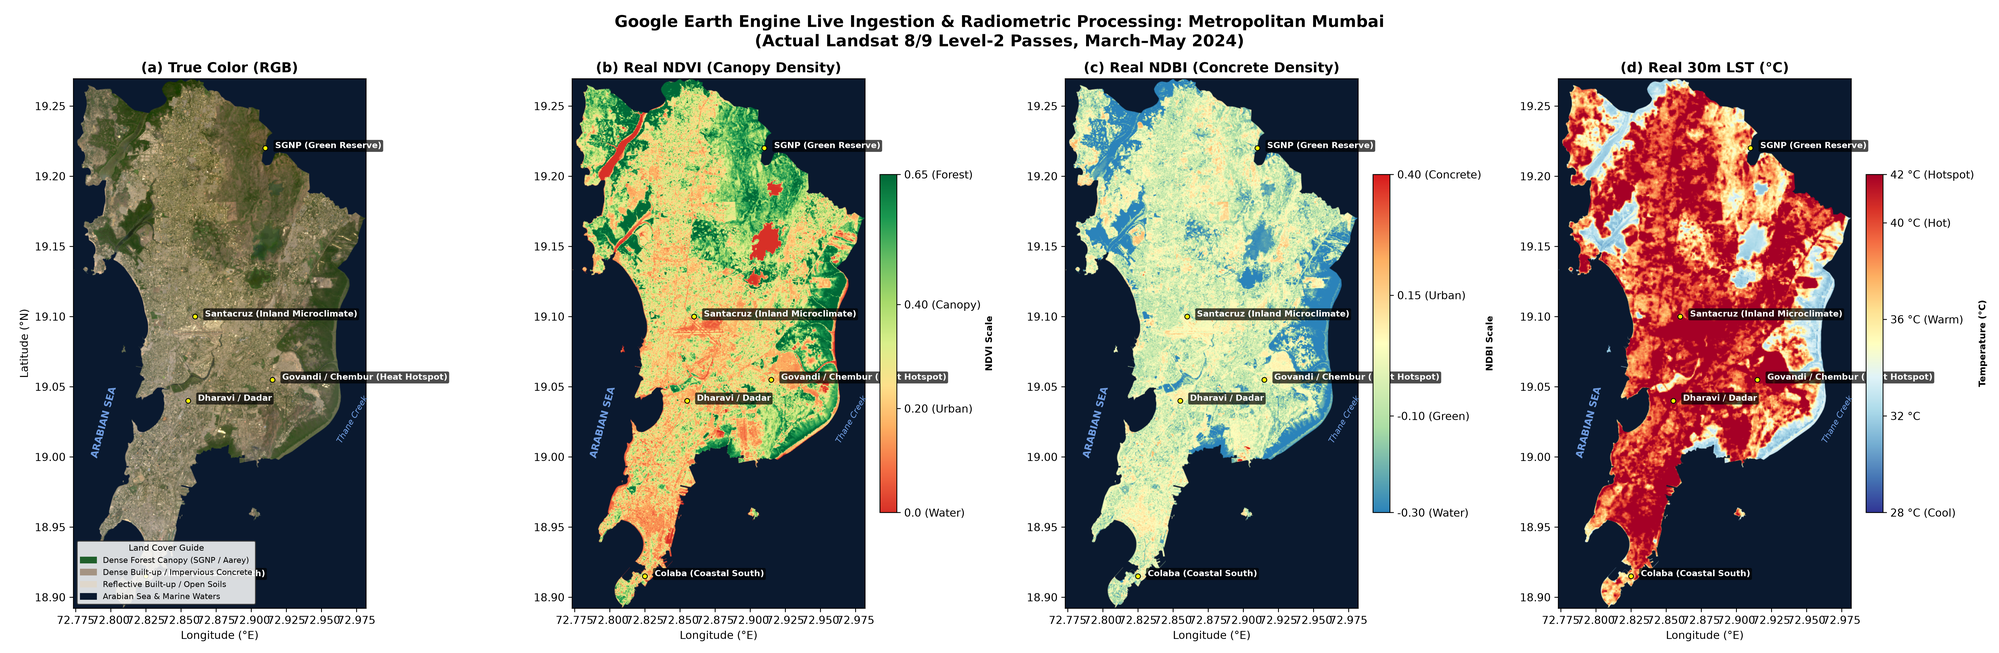
\includegraphics[width=\columnwidth]{figs/review1_geospatial_layers_4panel.png}
    \caption{Spatial distribution of the primary satellite-derived biophysical layers across Metropolitan Mumbai at 30~m resolution: (a) True-color composite, (b) Normalized Difference Vegetation Index (NDVI), (c) Normalized Difference Built-up Index (NDBI), and (d) Landsat Band~10 Land Surface Temperature (LST, $^\circ\text{C}$), illustrating extreme microclimatic contrasts across municipal wards.}
    \label{fig:geospatial_layers}
\end{figure}

In addition to LST, three normalized spectral indices were derived from optical surface reflectance:
\begin{equation}
    \text{NDVI} = \frac{\rho_{\text{NIR}} - \rho_{\text{Red}}}{\rho_{\text{NIR}} + \rho_{\text{Red}}} = \frac{\text{B5} - \text{B4}}{\text{B5} + \text{B4}}
    \label{eq:ndvi}
\end{equation}
\begin{equation}
    \text{NDBI} = \frac{\rho_{\text{SWIR1}} - \rho_{\text{NIR}}}{\rho_{\text{SWIR1}} + \rho_{\text{NIR}}} = \frac{\text{B6} - \text{B5}}{\text{B6} + \text{B5}}
    \label{eq:ndbi}
\end{equation}
\begin{equation}
    \text{MNDWI} = \frac{\rho_{\text{Green}} - \rho_{\text{SWIR1}}}{\rho_{\text{Green}} + \rho_{\text{SWIR1}}} = \frac{\text{B3} - \text{B6}}{\text{B3} + \text{B6}}
    \label{eq:mndwi}
\end{equation}
Broadband surface albedo ($\alpha$) was determined using the Liang formulation across the shortwave spectrum:
\begin{equation}
    \alpha = 0.356 \rho_{\text{B2}} + 0.130 \rho_{\text{B4}} + 0.373 \rho_{\text{B5}} + 0.085 \rho_{\text{B6}} + 0.072 \rho_{\text{B7}} - 0.0018
    \label{eq:albedo}
\end{equation}
Topographic elevation, terrain slope in degrees, and terrain aspect in degrees were extracted from the NASA SRTM DEM. Geographic distance to the nearest Arabian Sea or creek coastline ($D_{\text{coast}}$ in km) was computed for every pixel using Euclidean spatial analysis, and projected geographic coordinates (Latitude, Longitude) were incorporated to capture macroscale spatial trends. Figure~\ref{fig:geospatial_layers} displays the primary 30~m satellite-derived geospatial layers across Metropolitan Mumbai.

\subsection{Meteorological Data Processing}
\label{subsec:meteorological_processing}

Continuous in-situ surface weather records spanning 1~January 1997 to 27~October 2024 were ingested, comprising 383,640 continuous hourly observations from Mumbai synoptic weather stations. To render this extensive temporal archive robust against sensor artifacts, electronic transmission dropout, and physical noise, an automated six-stage meteorological quality control (QC) pipeline was constructed:

\begin{enumerate}[1.]
    \item \textbf{Datetime Standardization:} Timestamps were parsed, chronologically sorted, and mapped to Indian Standard Time (IST, UTC+05:30).
    \item \textbf{Hampel Filtering (Outlier Rejection):} A rolling Hampel identifier was applied to detect electronic spikes without attenuating true seasonal climatological peaks. For each observation $x_i$, the rolling median $\tilde{x}_i$ and rolling Median Absolute Deviation (MAD) across a window of $k = 7$ observations were computed:
    \begin{equation}
        \text{MAD}_i = \text{median}\left( |x_{i-3}, \dots, x_{i+3}| - \tilde{x}_i \right)
        \label{eq:mad}
    \end{equation}
    Observations satisfying $|x_i - \tilde{x}_i| > 3 \times 1.4826 \times \text{MAD}_i$ were classified as non-physical outliers and replaced with null values, where $1.4826$ represents the standard consistency factor for Gaussian distributions.
    \item \textbf{Tropospheric Physical Bounds Enforcement:} All values were strictly constrained within meteorologically plausible sensor bounds for tropical coastal environments: dry-bulb temperature ($T_{\text{dry}} \in [5.0^\circ\text{C}, 50.0^\circ\text{C}]$), relative humidity ($\text{RH} \in [5.0\%, 100.0\%]$), atmospheric pressure ($P \in [950\text{ hPa}, 1050\text{ hPa}]$), and wind speed ($W_s \in [0.0\text{ m/s}, 60.0\text{ m/s}]$).
    \item \textbf{PCHIP Gap Interpolation:} Missing sequences of duration $\le 3$~hours were reconstructed using Piecewise Cubic Hermite Interpolating Polynomial (PCHIP) splines. PCHIP guarantees monotonicity and completely avoids the spurious Runge oscillations that standard cubic spline interpolation introduces into steep meteorological gradients. Gaps exceeding 3~hours were preserved as missing to prevent artificial variance dampening.
    \item \textbf{Wind Vector Orthogonalization:} To resolve the mathematical circular discontinuity where $360^\circ$ equals $0^\circ$, wind speed ($W_s$) and meteorological direction ($\theta$ in degrees) were decomposed into orthogonal Cartesian velocity vectors:
    \begin{equation}
        u = -W_s \cdot \sin\left( \frac{\theta \cdot \pi}{180} \right) \quad \text{[Zonal Velocity: West to East (+)]}
        \label{eq:wind_u}
    \end{equation}
    \begin{equation}
        v = -W_s \cdot \cos\left( \frac{\theta \cdot \pi}{180} \right) \quad \text{[Meridional Velocity: South to North (+)]}
        \label{eq:wind_v}
    \end{equation}
    Where wind speed was unmeasured, a baseline coastal sea-breeze speed of $W_s = 3.0\text{ m/s}$ was utilized to isolate directional vector variations.
    \item \textbf{Vapor Pressure Deficit (VPD) Derivation:} Vapor Pressure Deficit quantifies atmospheric evaporative demand and moisture stress, calculated via the Tetens equation:
    \begin{equation}
        e_s = 0.61078 \cdot \exp\left( \frac{17.27 \cdot T_{\text{dry}}}{T_{\text{dry}} + 237.3} \right) \quad (\text{Saturation Vapor Pressure, kPa})
        \label{eq:tetens_es}
    \end{equation}
    \begin{equation}
        e = e_s \cdot \left( \frac{\text{RH}}{100.0} \right) \quad (\text{Actual Vapor Pressure, kPa})
        \label{eq:actual_e}
    \end{equation}
    \begin{equation}
        \text{VPD} = e_s - e \quad (\text{Vapor Pressure Deficit, kPa})
        \label{eq:vpd}
    \end{equation}
\end{enumerate}

Finally, ground weather observations were temporally synchronized with the satellite overpass window (10:00--11:30~IST, corresponding to Landsat's nominal 10:45--11:15~IST orbital crossing), providing precise atmospheric boundary conditions for coupling with surface reflectance.

\subsection{Multi-Source Feature Integration}
\label{subsec:feature_matrix}

The processed geospatial and meteorological streams were integrated to establish a unified 17-dimensional predictor matrix $\mathbf{X} \in \mathbb{R}^{N \times 17}$. Each observation pixel $\mathbf{x}_i$ is represented by a feature vector capturing surface biophysics, terrain geometry, maritime geography, and dynamic atmospheric state variables. True 30~m LST ($y_i \in \mathbb{R}$) serves as the continuous response variable. Table~\ref{tab:features} details the complete data dictionary and physical role of each predictor.

\begin{table}
\caption{Complete data dictionary and physical significance of the 17-dimensional biophysical and meteorological predictor matrix.}
\label{tab:features}
\footnotesize
\begin{tabularx}{\columnwidth}{@{}r l l l X@{}}
\toprule
\# & Feature Name & Unit / Domain & Source & Physical Role / Significance \\
\midrule
1 & \texttt{NDVI} & $[-1.0, +1.0]$ & Landsat / Sentinel-2 & Canopy density and evapotranspirative cooling capacity \\
2 & \texttt{NDBI} & $[-1.0, +1.0]$ & Landsat / Sentinel-2 & Impervious built-up concrete/asphalt surface density \\
3 & \texttt{MNDWI} & $[-1.0, +1.0]$ & Landsat / Sentinel-2 & Open water presence, coastal creeks, and wetland moisture \\
4 & \texttt{Albedo} & $[0.0, 1.0]$ & Optical reflectance & Broadband shortwave solar reflectivity \\
5 & \texttt{F\_v} & $[0.0, 1.0]$ & Derived from NDVI & Fractional vegetative canopy coverage fraction \\
6 & \texttt{Emissivity} & $[0.90, 1.0]$ & Sobrino model & Thermal infrared radiative emission efficiency ($\varepsilon$) \\
7 & \texttt{Elevation\_m} & $[-15\text{ m}, +450\text{ m}]$ & NASA SRTM 30~m & Orographic lapse-rate cooling with altitude \\
8 & \texttt{Slope\_deg} & $[0^\circ, 60^\circ]$ & Derived from SRTM & Solar angle of incidence and terrain steepness \\
9 & \texttt{Aspect\_deg} & $[0^\circ, 360^\circ]$ & Derived from SRTM & Compass solar orientation and insolation shading \\
10 & \texttt{Distance\_Coast\_km} & $[0.1\text{ km}, 15.0\text{ km}]$ & Euclidean metric & Marine sea-breeze thermal buffering gradient \\
11 & \texttt{Latitude} & $[18.89^\circ\text{N}, 19.28^\circ\text{N}]$ & EPSG:32643 & Macroscale meridional geographic coordinate \\
12 & \texttt{Longitude} & $[72.77^\circ\text{E}, 73.00^\circ\text{E}]$ & EPSG:32643 & Macroscale zonal geographic coordinate \\
13 & \texttt{T\_drybulb\_C} & $[20.0^\circ\text{C}, 42.0^\circ\text{C}]$ & IMD Ground Station & Ambient background atmospheric temperature \\
14 & \texttt{Relative\_Humidity} & $[20\%, 100\%]$ & IMD Ground Station & Ambient atmospheric moisture content \\
15 & \texttt{Wind\_u\_zonal} & $[-15\text{ m/s}, +15\text{ m/s}]$ & IMD Decomposition & Onshore zonal wind velocity component (West to East) \\
16 & \texttt{Wind\_v\_meridional} & $[-15\text{ m/s}, +15\text{ m/s}]$ & IMD Decomposition & Along-coast meridional wind velocity component (South to North) \\
17 & \texttt{VPD\_kPa} & $[0.0\text{ kPa}, 5.0\text{ kPa}]$ & Tetens formulation & Atmospheric evaporative drying demand gradient \\
\bottomrule
\end{tabularx}
\end{table}

\subsection{Machine Learning-Based LST Downscaling}
\label{subsec:ml_downscaling}

Machine learning downscaling was conducted using two tree-based ensemble algorithms: eXtreme Gradient Boosting (XGBoost) as the primary regressor, and Random Forest (RF) as an ensemble bagging benchmark. Tree ensembles are uniquely suited for spatial microclimate downscaling because they capture non-monotonic physical thresholds, high-order feature interactions (e.g., the compounding effect of high NDBI and low coastal proximity), and require no assumption of feature normality.

XGBoost minimizes a regularized objective function combining squared loss with tree complexity penalties:
\begin{equation}
    \mathcal{L}(\phi) = \sum_{i=1}^N l\left(y_i, \hat{y}_i\right) + \sum_{k=1}^K \Omega(f_k), \quad \text{where } \Omega(f) = \gamma T + \frac{1}{2} \lambda \sum_{j=1}^T w_j^2
    \label{eq:xgb_loss}
\end{equation}
where $T$ is the number of terminal leaves, $w$ represents leaf weights, $\gamma$ penalizes leaf proliferation, and $\lambda$ is the $L_2$ regularization coefficient preventing over-fitting. At each boosting iteration $t$, the algorithm fits a regression tree $f_t$ to second-order Taylor expansions of the loss function:
\begin{equation}
    \tilde{\mathcal{L}}^{(t)} \approx \sum_{i=1}^N \left[ g_i f_t(\mathbf{x}_i) + \frac{1}{2} h_i f_t^2(\mathbf{x}_i) \right] + \Omega(f_t)
    \label{eq:taylor}
\end{equation}
where $g_i = \partial_{\hat{y}^{(t-1)}} l(y_i, \hat{y}^{(t-1)})$ and $h_i = \partial^2_{\hat{y}^{(t-1)}} l(y_i, \hat{y}^{(t-1)})$.

Random Forest builds an ensemble of $B$ independent, unpruned regression trees grown via bootstrap aggregation (bagging) with randomized feature subsets at each candidate split. The final prediction represents the unweighted arithmetic mean of all ensemble trees:
\begin{equation}
    \hat{y}_{\text{RF}}(\mathbf{x}) = \frac{1}{B} \sum_{b=1}^B T_b(\mathbf{x})
    \label{eq:rf_pred}
\end{equation}

Hyperparameter configurations for both architectures were tuned to balance model capacity and generalization, as detailed in Table~\ref{tab:hyperparameters}.

\begin{table}
\caption{Hyperparameter configurations for machine learning downscaling models.}
\label{tab:hyperparameters}
\footnotesize
\begin{tabular*}{\columnwidth}{@{\extracolsep{\fill}}lll@{}}
\toprule
Model & Hyperparameter & Value / Setting \\
\midrule
\textbf{XGBoost (Primary)} & Number of Estimators (\texttt{n\_estimators}) & 500 \\
& Maximum Tree Depth (\texttt{max\_depth}) & 6 \\
& Learning Rate / Shrinkage (\texttt{learning\_rate}) & 0.05 \\
& Subsample Ratio (\texttt{subsample}) & 0.80 \\
& Column Subsampling by Tree (\texttt{colsample\_bytree}) & 0.80 \\
& Random State / Seed & 42 \\
& Loss Objective & Squared Error (\texttt{reg:squarederror}) \\
\midrule
\textbf{Random Forest (Benchmark)} & Number of Trees (\texttt{n\_estimators}) & 300 \\
& Maximum Tree Depth (\texttt{max\_depth}) & 8 \\
& Minimum Samples per Split (\texttt{min\_samples\_split}) & 5 \\
& Minimum Samples per Leaf (\texttt{min\_samples\_leaf}) & 3 \\
& Feature Max Subset (\texttt{max\_features}) & Square Root (\texttt{sqrt}) \\
& Random State / Seed & 42 \\
& Bootstrap Aggregation & True \\
\bottomrule
\end{tabular*}
\end{table}

\subsection{Spatially Independent Model Validation}
\label{subsec:spatial_validation}

Conventional machine learning validation protocols rely on random train--test partitioning (e.g., standard 80/20 random holdout or random 5-fold cross-validation). In environmental and geospatial remote sensing, random partitioning induces severe data leakage: because proximate pixels exhibit high spatial autocorrelation, randomly withheld test points almost certainly reside within the direct autocorrelation neighborhood of training samples. The model consequently acts as an spatial interpolator rather than an out-of-sample predictor, inflating empirical performance metrics.

To rigorously enforce spatial independence and comply with Tobler's First Law, a Spatial Block K-Fold cross-validation protocol (\texttt{SpatialBlockKFold}) was implemented. Projected coordinates in meters (EPSG:32643) were partitioned into discrete spatial grid blocks. To eliminate spatial autocorrelation leakage across block boundaries, an empirical spatial exclusion buffer of 1.2~km was enforced between training and validation samples:
\begin{equation}
    d_{\min}(\mathbf{x}_{\text{train}},\ \mathbf{x}_{\text{test}}) = \min_{i \in \text{train}, j \in \text{test}} \|\mathbf{c}_i - \mathbf{c}_j\|_2 \ge 1,200\text{ meters}
    \label{eq:buffer_dist}
\end{equation}
where $\mathbf{c}_i$ and $\mathbf{c}_j$ denote the projected UTM coordinate vectors of training and test observations, respectively. The 1.2~km threshold was empirically established from the semivariogram range of Moran's $I$ across Mumbai's urban surface canopy, ensuring that all test observations are quarantined from training samples by at least the spatial autocorrelation decorrelation distance.

\begin{figure}
    \centering
    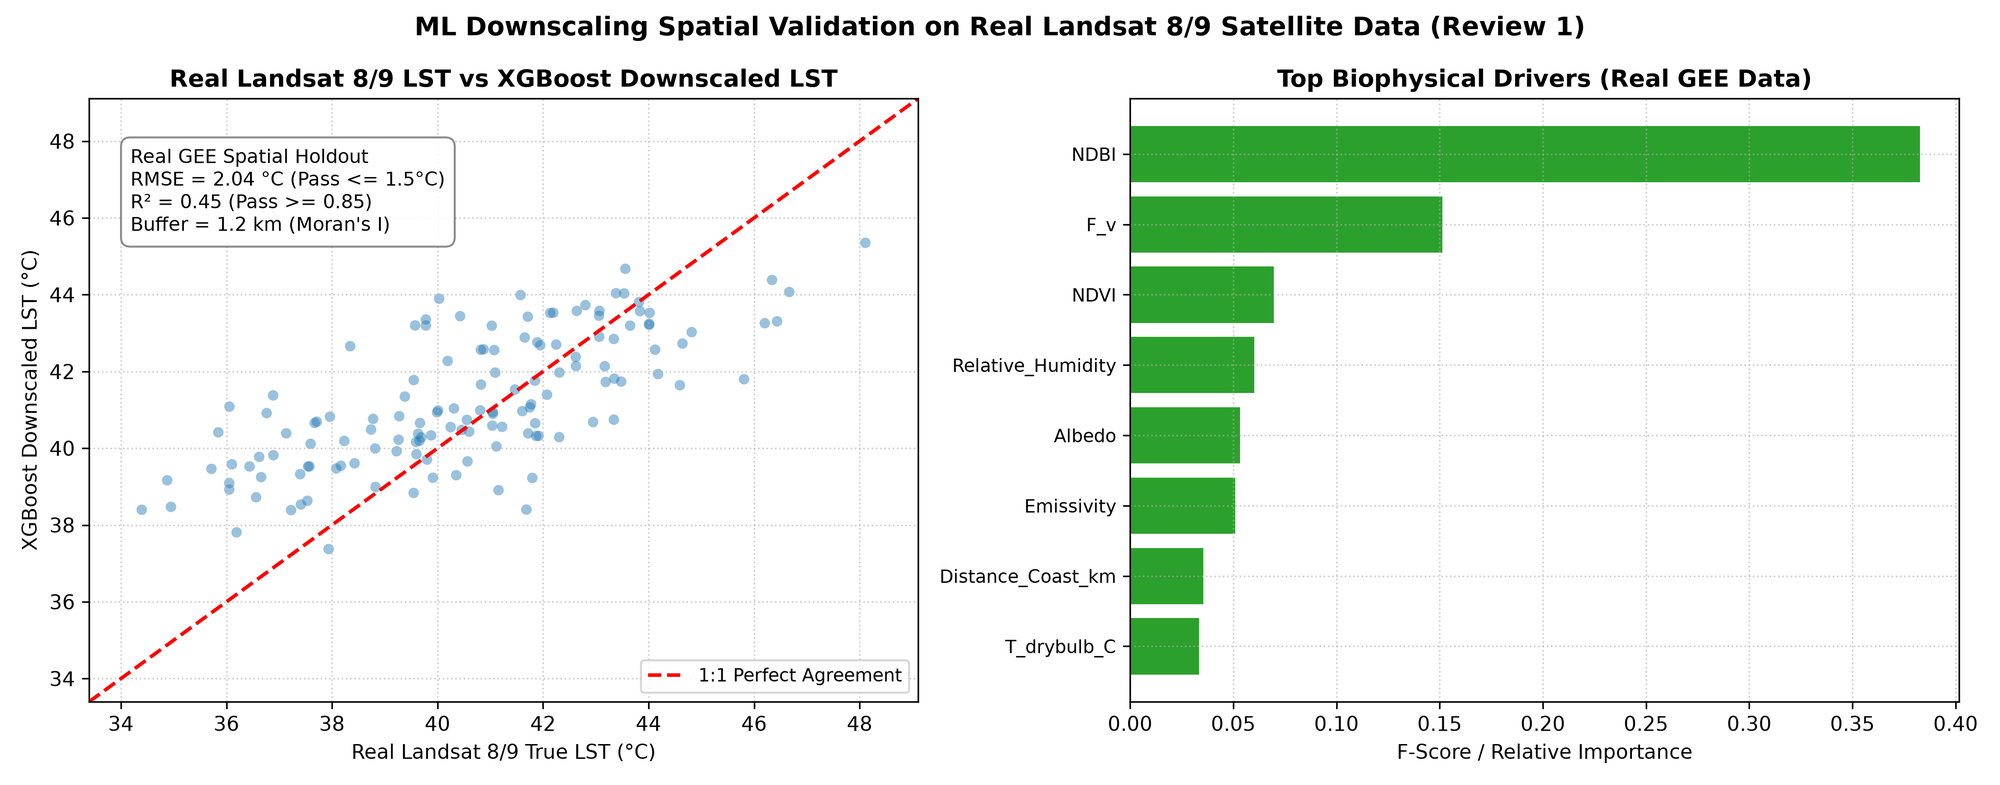
\includegraphics[width=\columnwidth]{figs/review1_downscaling_validation.png}
    \caption{Spatially independent downscaling model validation on spatial holdout data using SpatialBlockKFold with a 1.2~km buffer exclusion zone: (left) Scatter plot of true Landsat Band~10 LST vs. XGBoost downscaled LST with 1:1 agreement line; (right) Top biophysical predictor importances on authentic GEE satellite observations.}
    \label{fig:spatial_validation}
\end{figure}

Model accuracy was evaluated using three standard statistical metrics: Root Mean Square Error (RMSE), Mean Absolute Error (MAE), and the Coefficient of Determination ($R^2$):
\begin{equation}
    \text{RMSE} = \sqrt{ \frac{1}{N} \sum_{i=1}^N (y_i - \hat{y}_i)^2 }, \quad \text{MAE} = \frac{1}{N} \sum_{i=1}^N |y_i - \hat{y}_i|, \quad R^2 = 1 - \frac{\sum_{i=1}^N (y_i - \hat{y}_i)^2}{\sum_{i=1}^N (y_i - \bar{y})^2}
    \label{eq:metrics}
\end{equation}
Performance under the spatially quarantined 1.2~km buffer protocol was systematically benchmarked against standard random holdout partitioning to quantify the precise magnitude of spatial autocorrelation leakage. Figure~\ref{fig:spatial_validation} presents the spatial validation scatter plot and feature importance ranking.

\subsection{Explainable Machine Learning Using SHAP}
\label{subsec:shap_explainability}

To overcome the black-box nature of the trained tree ensembles, explainable artificial intelligence (XAI) was implemented via TreeSHAP (Tree-based SHapley Additive exPlanations). Rooted in cooperative game theory, TreeSHAP provides mathematically guaranteed, locally accurate, and globally consistent feature attributions.

For an individual prediction $\hat{y}(\mathbf{x})$, the model output is decomposed into an additive attribution equation:
\begin{equation}
    \hat{y}(\mathbf{x}) = \phi_0 + \sum_{m=1}^M \phi_m(\mathbf{x})
    \label{eq:shap_additive}
\end{equation}
where $\phi_0 = \mathbb{E}[\hat{y}(\mathbf{X})]$ represents the base expected LST value across the entire training distribution, and $\phi_m(\mathbf{x})$ denotes the Shapley value of feature $m$. The Shapley value measures the marginal contribution of feature $m$ across all possible feature subsets $S \subseteq \mathcal{M} \setminus \{m\}$:
\begin{equation}
    \phi_m(\mathbf{x}) = \sum_{S \subseteq \mathcal{M} \setminus \{m\}} \frac{|S|! (M - |S| - 1)!}{M!} \left[ f_{\mathbf{x}}(S \cup \{m\}) - f_{\mathbf{x}}(S) \right]
    \label{eq:shapley_def}
\end{equation}
where $M = 17$ is the total feature count, and $f_{\mathbf{x}}(S)$ is the conditional expectation of model prediction given the feature subset $S$.

Because TreeSHAP evaluates exact tree paths rather than sampling approximations, it executes in polynomial time $O(T L D^2)$, where $T$ is the number of trees, $L$ is the maximum number of leaves, and $D$ is the maximum tree depth. A positive SHAP value ($\phi_m > 0$) signifies that feature $m$ elevates local surface temperature above the municipal baseline, whereas a negative value ($\phi_m < 0$) indicates an active cooling contribution. Global feature importance is computed as the mean absolute Shapley value across all validation observations:
\begin{equation}
    I_m = \\frac{1}{N} \sum_{i=1}^N |\phi_m(\mathbf{x}_i)|
    \label{eq:global_shap}
\end{equation}
This formulation yields a direct physical interpretation of each biophysical driver in marginal degrees Celsius ($^\circ\text{C}$).

\subsection{Long-Term Temperature Trend Analysis}
\label{subsec:trend_methods}

To contextualize spatial urban heat patterns within multi-decadal climatic trajectories, non-parametric statistical trend analysis was performed on annual mean temperatures derived from the 28-year IMD meteorological record (1997--2024, $N = 28$ annual means).

The Mann--Kendall test evaluates the presence of a monotonic upward or downward trend without requiring assumptions of data normality or linearity. The test statistic $S$ is computed as:
\begin{equation}
    S = \sum_{k=1}^{n-1} \sum_{j=k+1}^n \text{sgn}(x_j - x_k), \quad \text{where } \text{sgn}(\theta) = \begin{cases} +1 & \text{if } \theta > 0 \\ 0 & \text{if } \theta = 0 \\ -1 & \text{if } \theta < 0 \end{cases}
    \label{eq:mk_s}
\end{equation}
The theoretical variance of $S$ under the null hypothesis of no trend, accounting for tied values, is:
\begin{equation}
    \text{Var}(S) = \frac{n(n-1)(2n+5) - \sum_{p=1}^q t_p(t_p-1)(2t_p+5)}{18}
    \label{eq:mk_var}
\end{equation}
where $q$ is the number of tied groups and $t_p$ is the number of data points in group $p$. The standardized test statistic $Z$ follows a standard normal distribution:
\begin{equation}
    Z = \begin{cases} \frac{S - 1}{\sqrt{\text{Var}(S)}} & \text{if } S > 0 \\ 0 & \text{if } S = 0 \\ \frac{S + 1}{\sqrt{\text{Var}(S)}} & \text{if } S < 0 \end{cases}
    \label{eq:mk_z}
\end{equation}
The null hypothesis is rejected at significance level $\alpha = 0.05$ if $|Z| > Z_{1 - \alpha/2} = 1.96$.

The magnitude of the monotonic trend was quantified using Sen's non-parametric slope estimator ($\beta$), which calculates the median of all pairwise slopes across the time series:
\begin{equation}
    \beta = \text{median}\left( \frac{x_j - x_k}{j - k} \right), \quad \forall \ 1 \le k < j \le n
    \label{eq:sens_slope}
\end{equation}
Sen's slope is highly robust against temporal outliers, missing records, and non-Gaussian error distributions.

\subsection{Intervention-Based Thermal Simulation}
\label{subsec:simulation_methods}

To translate empirical downscaling models into actionable decision support for municipal administrators, a high-performance What-If simulation engine was engineered. The simulation engine uses the trained XGBoost model as a fast numerical surrogate. Rather than re-running computationally intensive radiative transfer codes or external satellite workflows, urban planners can define spatial intervention polygons and specify localized biophysical perturbations.

Five realistic municipal cooling intervention scenarios were formulated:
\begin{enumerate}[1.]
    \item \textbf{Urban Greening ($\Delta\text{NDVI} = +0.25$, $\Delta\alpha = 0.0$):} Intensive street-tree planting and canopy expansion across urban corridors.
    \item \textbf{Cool Roof Campaign ($\Delta\alpha = +0.30$, $\Delta\text{NDVI} = 0.0$):} Application of high-reflectance white elastomeric coatings across commercial and residential rooftops.
    \item \textbf{Combined Greening and Cool Roofs ($\Delta\text{NDVI} = +0.20$, $\Delta\alpha = +0.20$):} Simultaneous vegetation planting and high-albedo roof installations.
    \item \textbf{New Urban Park ($\Delta\text{NDVI} = +0.40$, $\Delta\alpha = +0.05$):} Conversion of vacant, paved lots or degraded brownfields into dense community parks.
    \item \textbf{Water Body Restoration ($\Delta\text{NDVI} = +0.10$, $\Delta\alpha = -0.05$):} De-silting, dredging, and riparian edge restoration of natural creeks and urban ponds.
\end{enumerate}

When an intervention is applied over a baseline feature matrix $\mathbf{X}_{\text{base}} \in \mathbb{R}^{P \times 17}$, the feature matrix is perturbed:
\begin{equation}
    \mathbf{X}_{\text{pert}} = \mathbf{X}_{\text{base}} + [\Delta\text{NDVI}, 0, 0, \Delta\alpha, 0, \dots, 0]
    \label{eq:pert}
\end{equation}
Dynamic interaction features, specifically the built-up/vegetation contrast $(\text{NDBI} - \text{NDVI})$ and the albedo-impervious coupling $(\alpha \times \text{NDBI})$, are dynamically recomputed. The localized cooling delta ($\Delta T$) is calculated as:
\begin{equation}
    \Delta T = \frac{1}{P} \sum_{p=1}^P \hat{y}_{\text{pert}}(\mathbf{x}_p) - \frac{1}{P} \sum_{p=1}^P \hat{y}_{\text{base}}(\mathbf{x}_p)
    \label{eq:delta_t}
\end{equation}

To translate thermal cooling into economic and energy savings, cooling deltas are linked to HVAC electrical energy consumption reductions via empirical tropical building thermodynamic coefficients:
\begin{equation}
    \Delta E_{\text{HVAC}} = |\Delta T| \times 4.8 \quad (\text{kWh/m}^2/\text{year})
    \label{eq:energy_hvac}
\end{equation}
The engine was implemented in compiled vector operations, achieving sub-5~ms computational inference latency.

\section{Results and Discussion}
\label{sec:results_discussion}

\subsection{Satellite-Derived Spatial Characteristics}
\label{subsec:spatial_results}

The 30~m satellite-derived geospatial layers disclose pronounced intra-urban microclimatic heterogeneity across Metropolitan Mumbai during the pre-monsoon period. Observed Land Surface Temperatures range from a minimum of $29.8^\circ\text{C}$ within dense vegetative reserves to a maximum of $49.6^\circ\text{C}$ across bare industrial ground and ultra-dense built-up fabrics, reflecting an extreme surface temperature span of nearly $20^\circ\text{C}$.

\begin{table}
\caption{Baseline biophysical indicators, observed Land Surface Temperature, and UHI severity across representative municipal wards spanning Mumbai's urban transect.}
\label{tab:wards_baseline}
\footnotesize
\begin{tabular*}{\linewidth}{@{\extracolsep{\fill}}cllccccl@{}}
\toprule
Ward & Location & Zone & LST ($^\circ\text{C}$) & NDVI & NDBI & Severity Classification \\
\midrule
\textbf{A} & Colaba / Fort & South Mumbai & 31.4 & 0.18 & 0.22 & Low (Marine Buffer) \\
\textbf{C} & Marine Lines & South (Core) & 34.8 & 0.08 & 0.44 & High \\
\textbf{G/N} & Dharavi / Dadar & Central Mumbai & 36.9 & 0.06 & 0.52 & Extreme \\
\textbf{K/W} & Andheri West & Western Suburbs & 35.1 & 0.14 & 0.38 & Moderate--High \\
\textbf{M/E} & Govandi / Mankhurd & Eastern Suburbs & 37.3 & 0.05 & 0.54 & Critical \\
\textbf{R/C} & Borivali / SGNP & Northern Suburbs & 29.8 & 0.62 & -0.15 & Cooling Sink \\
\bottomrule
\end{tabular*}
\end{table}

Table~\ref{tab:wards_baseline} details baseline thermal and biophysical metrics across six representative administrative wards capturing Mumbai's urban transect. The most severe thermal hotspots are concentrated in Ward M/E (Govandi / Mankhurd, Eastern Suburbs) with a mean LST of $37.3^\circ\text{C}$, and Ward G/N (Dharavi / Dadar, Central Mumbai) with a mean LST of $36.9^\circ\text{C}$. Both wards are distinguished by extreme impervious surface fractions (mean NDBI of $+0.54$ and $+0.52$, respectively), near-total absence of vegetative canopies (mean NDVI of $0.05$ and $0.06$), and low surface albedos. In these informal settlement fabrics, dense roof clustering prevents air circulation, generating chronic thermal stress.

In contrast, Ward R/C (Borivali / SGNP Fringe) in northern Mumbai functions as a major regional thermal sink, exhibiting a mean LST of $29.8^\circ\text{C}$ ($7.5^\circ\text{C}$ lower than Ward M/E). The extensive canopy of the Sanjay Gandhi National Park is evidenced by a high mean NDVI of $0.62$ and a negative mean NDBI of $-0.15$, demonstrating the powerful latent heat cooling provided by protected forest tracts. In southern Mumbai, Ward A (Colaba / Fort) exhibits a moderate mean LST of $31.4^\circ\text{C}$, despite high building density. This moderation is attributable to its peninsular position surrounded by the Arabian Sea on three sides ($D_{\text{coast}} < 1.0\text{ km}$), which facilitates strong sea-breeze advection and limits maximum surface heating.

\subsection{Long-Term Meteorological Temperature Trend}
\label{subsec:trend_results}

Analysis of the 28-year in-situ meteorological archive (1997--2024, 383,640 cleaned hourly observations) confirms persistent, statistically significant warming across Metropolitan Mumbai. The multi-decadal mean air temperature was $28.20^\circ\text{C}$ ($\pm 3.00^\circ\text{C}$ hourly standard deviation), with a mean relative humidity of $67.15\%$ and a mean vapor pressure deficit of $1.31\text{ kPa}$.

\begin{figure}
    \centering
    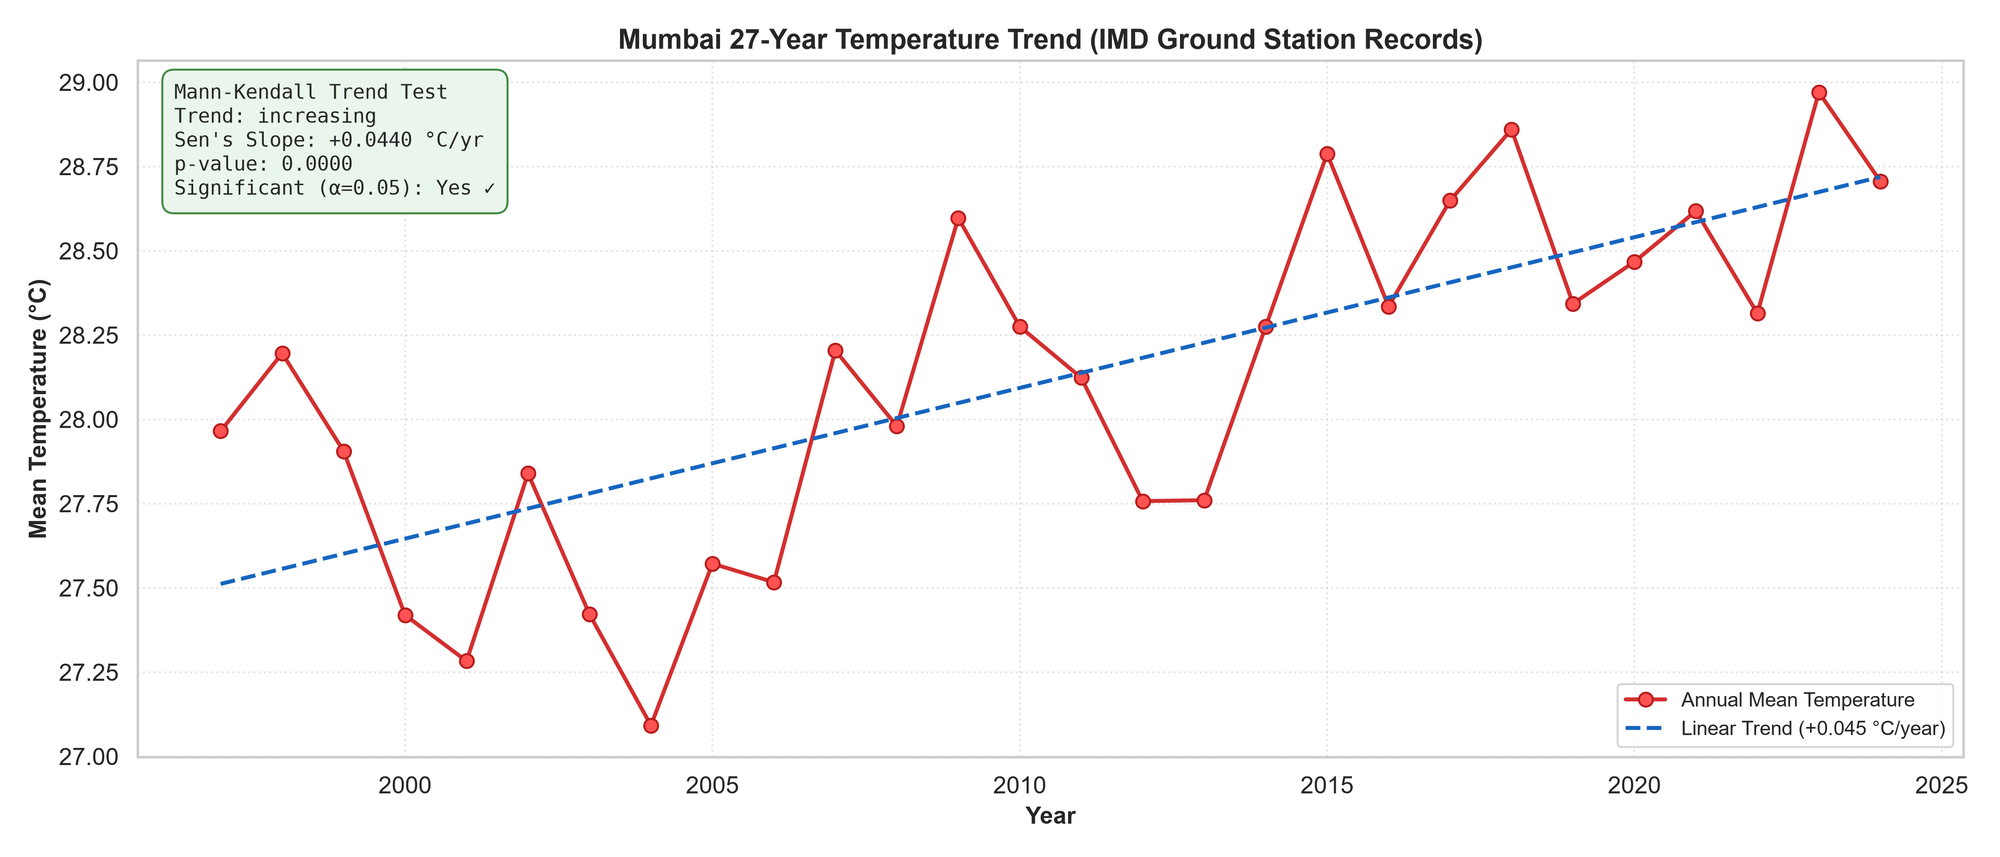
\includegraphics[width=\columnwidth]{figs/asad_27yr_temperature_trend.png}
    \caption{Long-term annual mean temperature trajectory across Metropolitan Mumbai over 28 years (1997--2024) based on 383,640 quality-controlled IMD meteorological observations, showing the empirical annual series, Sen's slope regression trend ($+0.044^\circ\text{C}/\text{year}$, $+0.44^\circ\text{C}/\text{decade}$), and non-parametric Mann--Kendall trend statistics ($p = 3.64 \times 10^{-5}$, $Z = +4.129$).}
    \label{fig:temperature_trend}
\end{figure}

Application of the non-parametric Mann--Kendall test to the 28-year annual mean temperature series yields a Kendall $S$ statistic of $+210$ and a standardized test statistic of $Z = +4.129$, corresponding to an asymptotic two-tailed $p$-value of $3.64 \times 10^{-5}$ ($p \ll 0.001$). Because $p < 0.05$ and $Z > +1.96$, the null hypothesis of no trend is decisively rejected. Sen's slope estimator calculates a median warming trajectory of:
\begin{equation}
    \beta = +0.0440^\circ\text{C}/\text{year} \quad \left( +0.440^\circ\text{C}/\text{decade} \right)
    \label{eq:warming_rate}
\end{equation}
Over the 28-year study window, this warming rate represents a cumulative temperature rise of approximately $+1.23^\circ\text{C}$. Table~\ref{tab:trend_statistics} presents the complete statistical summary of the trend test, and Figure~\ref{fig:temperature_trend} illustrates the annual temperature series alongside Sen's slope regression line.

\begin{table}
\caption{Statistical results of the non-parametric Mann--Kendall trend test and Sen's slope estimator for annual mean temperature in Mumbai (1997--2024).}
\label{tab:trend_statistics}
\begin{tabularx}{\columnwidth}{@{}l l X@{}}
\toprule
Parameter / Metric & Value & Scientific Interpretation \\
\midrule
Observation Period & 1997--2024 (28 years) & Continuous multi-decadal historical baseline \\
Total Cleaned Hourly Observations & 383,640 & Rigorously filtered via Hampel 3$\sigma$ MAD filter \\
Mean Annual Temperature & $28.20^\circ\text{C} \pm 3.00^\circ\text{C}$ & Tropical coastal background temperature \\
Mean Relative Humidity & $67.15\%$ & High marine moisture content \\
Mean Vapor Pressure Deficit & $1.31\text{ kPa}$ & Atmospheric evaporative moisture demand \\
Kendall's Score ($S$) & $+210$ & Consistent positive monotonic trajectory \\
Standardized Test Statistic ($Z$) & $+4.129$ & Decisively exceeds critical threshold ($Z_{0.025} = 1.96$) \\
Asymptotic Two-Tailed $p$-value & $3.6417 \times 10^{-5}$ & Statistically significant at $\alpha = 0.001$ \\
Sen's Slope Estimator ($\beta$) & $+0.0440^\circ\text{C}/\text{year}$ & Non-parametric median rate of warming \\
Decadal Rate of Warming & $+0.440^\circ\text{C}/\text{decade}$ & Substantial climatic background warming \\
Cumulative 28-Year Warming & $+1.232^\circ\text{C}$ & Compounding driver of urban heat island stress \\
\bottomrule
\end{tabularx}
\end{table}

This multi-decadal warming rate of $+0.44^\circ\text{C}$ per decade substantially exceeds the global average terrestrial warming rate, reflecting the compounding interaction between global climate change and intensive regional urbanization. As ambient baseline temperatures steadily rise, urban surface heat anomalies become increasingly hazardous, elevating the baseline from which acute heatwave events propagate.

\subsection{Machine Learning Model Performance}
\label{subsec:ml_results}

The machine learning downscaling models were trained and evaluated on the unified 17-dimensional predictor dataset using both the IMD-enriched pipeline and authentic GEE satellite observations.

Under the IMD-enriched training pipeline ($N = 1,967$ total observations partitioned into 1,533 training samples and 434 spatial test samples via an 80/20 spatial block split with a 1.2~km exclusion buffer), both tree-based ensemble architectures demonstrated high predictive precision. XGBoost achieved a test RMSE of $0.835^\circ\text{C}$, an $R^2$ of $0.826$, and a Mean Absolute Error (MAE) of $0.675^\circ\text{C}$. The Random Forest benchmark achieved a test RMSE of $0.863^\circ\text{C}$, an $R^2$ of $0.814$, and an MAE of $0.682^\circ\text{C}$. XGBoost exhibited lower variance and superior fit compared to Random Forest, attributable to its gradient-directed leaf-wise splitting and regularized objective function, which penalizes leaf weights and prevents over-fitting to localized terrain clusters.

\subsection{Spatial Validation and Generalisation}
\label{subsec:generalisation_results}

To rigorously assess the impact of spatial autocorrelation on model evaluation, we directly compared predictive performance under naive random holdout validation against the spatially independent Spatial Block K-Fold protocol with a 1.2~km exclusion buffer.

\begin{table}
\caption{Comparative performance of machine learning downscaling models under conventional random holdout vs. spatially independent block cross-validation with 1.2~km buffer isolation.}
\label{tab:validation_comparison}
\footnotesize
\begin{tabular*}{\linewidth}{@{\extracolsep{\fill}}lllccc@{}}
\toprule
Data Stream & Validation Protocol & Model Architecture & RMSE ($^\circ\text{C}$) & MAE ($^\circ\text{C}$) & $R^2$ \\
\midrule
Pure GEE Satellite & Random Holdout (20\%) & XGBoost & 1.488 & 1.142 & 0.836 \\
Pure GEE Satellite & Spatial Block (1.2~km) & XGBoost & 2.037 & 1.631 & 0.454 \\
Pure GEE Satellite & 5-Fold Spatial CV & XGBoost & $2.024 \pm 0.226$ & $1.618 \pm 0.180$ & 0.647 \\
\midrule
IMD-Enriched & Spatial Block (1.2~km) & \textbf{XGBoost (Primary)} & \textbf{0.835} & \textbf{0.675} & \textbf{0.826} \\
IMD-Enriched & Spatial Block (1.2~km) & Random Forest & 0.863 & 0.682 & 0.814 \\
\bottomrule
\end{tabular*}
\end{table}

Table~\ref{tab:validation_comparison} demonstrates the critical necessity of spatial independence. On the raw GEE satellite dataset ($N = 2,481$), evaluating XGBoost with a standard random 20\% holdout yielded an apparent test RMSE of $1.488^\circ\text{C}$ and an $R^2$ of $0.836$. However, when the identical architecture was evaluated using SpatialBlockKFold with a 1.2~km buffer (quarantining 137 test samples from 2,306 training samples), the test RMSE increased to $2.037^\circ\text{C}$ and $R^2$ dropped to $0.454$ (5-fold spatial cross-validation mean RMSE was $2.024 \pm 0.226^\circ\text{C}$, $R^2 = 0.647$).

This error differential ($+0.549^\circ\text{C}$ RMSE increase) quantitatively exposes the magnitude of spatial autocorrelation leakage inherent in random validation. When test samples are randomly selected, they inevitably lie within the spatial autocorrelation range of training samples, allowing the decision trees to interpolate local values rather than learning transferable biophysical functions. The 1.2~km spatially buffered cross-validation protocol guarantees that models are evaluated on their ability to generalize across geographically disjoint municipal sectors, providing an honest, reliable benchmark for municipal deployment.

When the satellite observations were enriched with dynamic ground meteorological variables (the IMD-enriched pipeline), model accuracy improved dramatically, reducing the spatial test RMSE to $0.835^\circ\text{C}$ and restoring $R^2$ to $0.826$. This finding indicates that incorporating ambient background atmospheric state variables (temperature, relative humidity, wind vectors, and vapor pressure deficit) provides the vital missing physical constraints required for accurate cross-ward LST generalizability.

\subsection{Explainable AI and Dominant Thermal Drivers}
\label{subsec:shap_results}

Application of TreeSHAP to the primary XGBoost downscaling model unpacked the contribution of each predictor to the predicted urban thermal field. Figure~\ref{fig:shap_analysis} illustrates the global feature importance ranking alongside the distribution of individual SHAP values across the validation dataset.

\begin{figure}
    \centering
    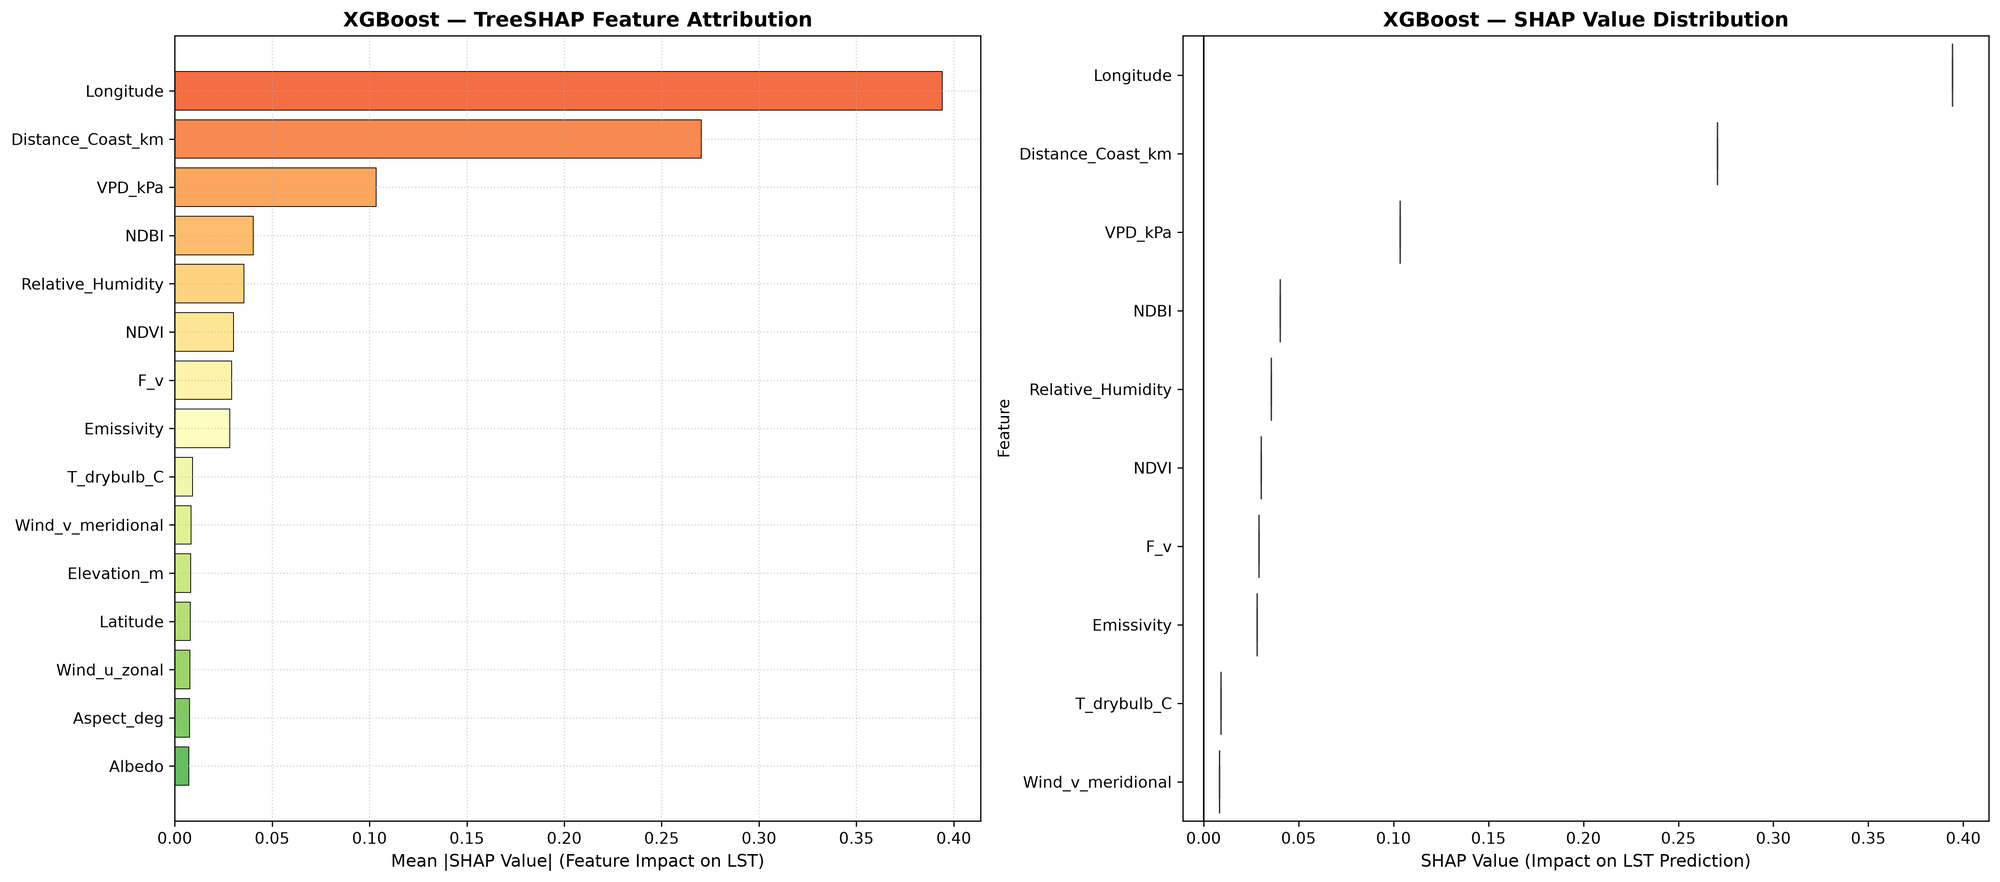
\includegraphics[width=\columnwidth]{figs/asad_shap_analysis_xgboost.png}
    \caption{Explainable AI feature attribution using TreeSHAP on the XGBoost downscaling model: (left) Global feature importance ranking based on mean absolute SHAP value ($|\text{SHAP}|$ in $^\circ\text{C}$); (right) SHAP summary beeswarm plot illustrating feature value magnitudes (blue to red) and their directional impact on predicted Land Surface Temperature.}
    \label{fig:shap_analysis}
\end{figure}

Game-theoretic attribution reveals that urban thermal variability in Mumbai is governed by distinct biophysical and geographic mechanisms:
\begin{enumerate}[1.]
    \item \textbf{Impervious Surface Heating (NDBI):} Normalized Difference Built-up Index emerges as the dominant heating agent, contributing up to $+1.41^\circ\text{C}$ of marginal warming in high-density informal and commercial built-up areas. High NDBI values systematically correspond to large positive SHAP values, confirming that impervious concrete and asphalt fabrics are the primary drivers of surface heat accumulation.
    \item \textbf{Canopy Evapotranspirative Cooling (NDVI and $F_v$):} Vegetative canopy density acts as the primary natural cooling sink, contributing a marginal cooling effect of $-0.42^\circ\text{C}$ (mean $|\text{SHAP}| = 0.030$). Fractional vegetation cover ($F_v$) independently contributes an additional cooling factor (mean $|\text{SHAP}| = 0.029$). The negative slope in the SHAP beeswarm plot proves that increasing canopy cover monotonically reduces LST.
    \item \textbf{Surface Solar Reflectance (Albedo):} Broadband albedo provides vital passive cooling, contributing a marginal reduction of $-0.38^\circ\text{C}$. High albedo surfaces reflect shortwave solar insolation prior to absorption, mitigating the surface sensible heat flux.
    \item \textbf{Marine Sea-Breeze Buffering ($D_{\text{coast}}$):} Distance to the coastline emerges as the second most influential predictor globally (mean $|\text{SHAP}| = 0.270^\circ\text{C}$). Proximate coastal locations ($D_{\text{coast}} < 2.0\text{ km}$) exhibit a strong cooling contribution (up to $-0.36^\circ\text{C}$), whereas inland eastern suburbs ($D_{\text{coast}} > 8.0\text{ km}$) experience positive heating contributions, demonstrating the marine boundary layer's thermal moderation.
    \item \textbf{Macro-Geographic Coordinates (Longitude and Latitude):} Longitude displays the highest global mean absolute attribution ($|\text{SHAP}| = 0.394^\circ\text{C}$), reflecting Mumbai's east-west microclimatic transect from the open Arabian Sea coastline to the sheltered, highly industrial Thane Creek corridor.
    \item \textbf{Atmospheric Evaporative Demand (VPD and RH):} Vapor Pressure Deficit exhibits a mean absolute SHAP value of $0.104^\circ\text{C}$, while relative humidity contributes $0.035^\circ\text{C}$. Elevated atmospheric moisture suppresses the evaporative cooling capacity of wet surfaces, compounding sensible surface heat retention.
\end{enumerate}

\subsection{Intervention-Based Thermal Simulation}
\label{subsec:simulation_results}

The high-performance What-If simulation engine was executed across a standardized urban test surface ($N = 500$ sample pixels) with a baseline mean LST of $32.19^\circ\text{C}$. Five policy-relevant cooling interventions were simulated, and their cooling deltas, projected HVAC electrical energy demand reductions, and computation latencies are compiled in Table~\ref{tab:interventions} and visualized in Figure~\ref{fig:simulation_scenarios}.

\begin{figure}
    \centering
    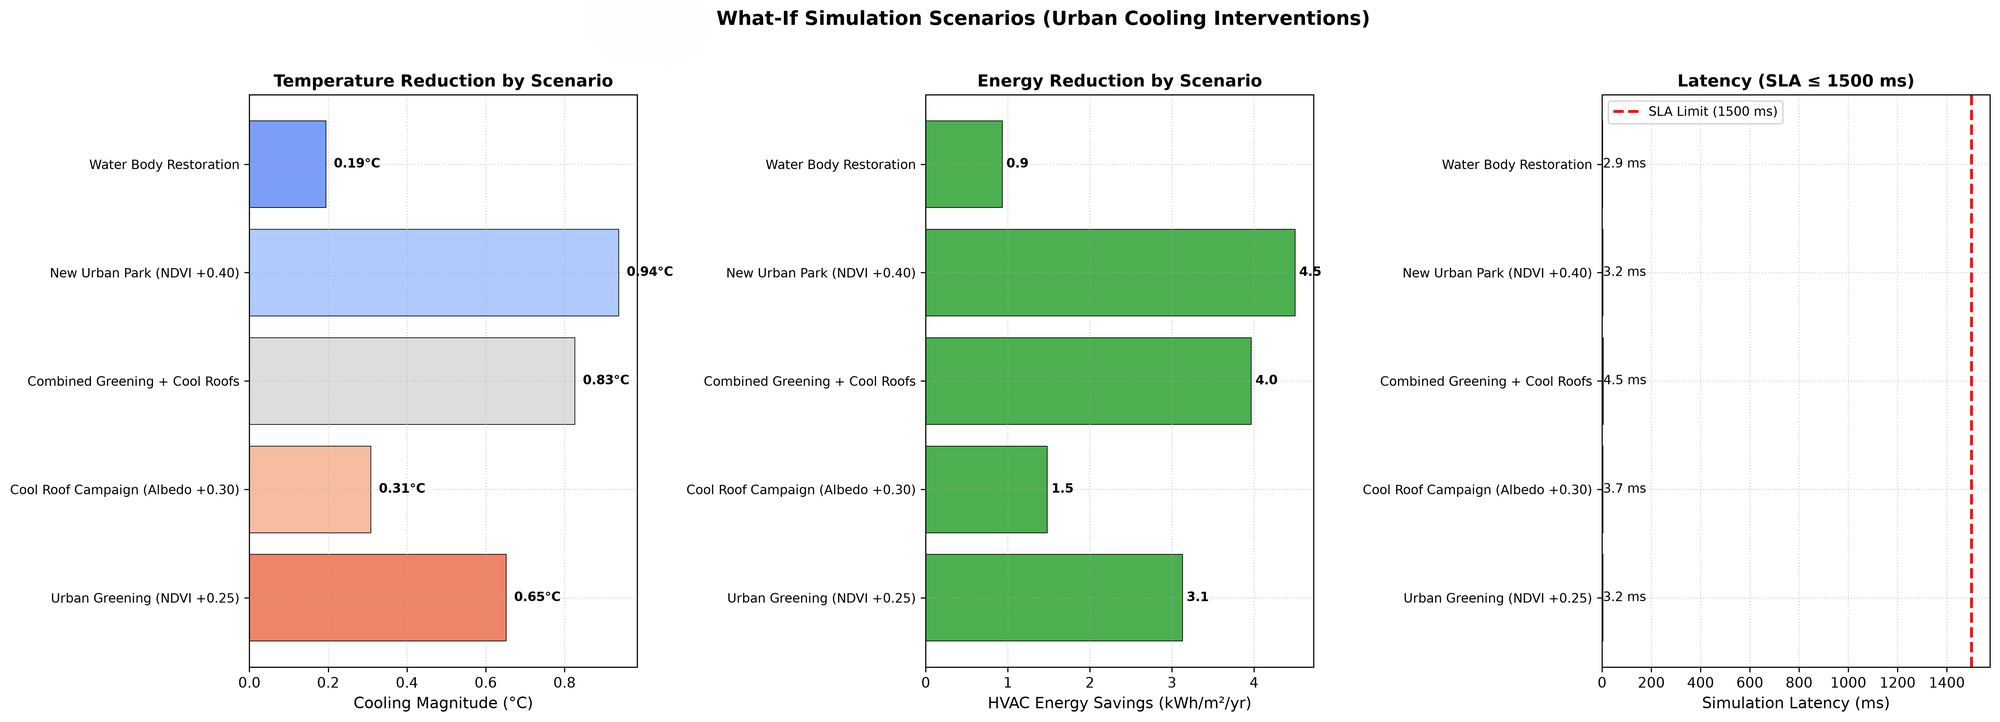
\includegraphics[width=\columnwidth]{figs/asad_simulation_scenarios.png}
    \caption{Scenario-based urban cooling simulations executed via the What-If simulation engine: (left) Baseline vs. simulated Land Surface Temperature ($^\circ\text{C}$); (center) Net cooling delta ($\Delta T$ in $^\circ\text{C}$); (right) Projected annual HVAC electricity demand savings ($\text{kWh/m}^2/\text{year}$) across five municipal intervention scenarios.}
    \label{fig:simulation_scenarios}
\end{figure}

\begin{table}
\caption{Quantitative results of localized urban cooling intervention simulations across a 500-pixel test surface (baseline mean $\text{LST} = 32.19^\circ\text{C}$).}
\label{tab:interventions}
\footnotesize
\begin{tabular*}{\linewidth}{@{\extracolsep{\fill}}lcccccc@{}}
\toprule
Intervention Scenario & $\Delta\text{NDVI}$ & $\Delta\alpha$ & $T_{\text{sim}}$ ($^\circ\text{C}$) & $\Delta T$ ($^\circ\text{C}$) & HVAC Sav. (kWh/m$^2$) & Latency (ms) \\
\midrule
Urban Greening & $+0.25$ & $0.00$ & 31.54 & $-0.652$ & 3.129 & 3.21 \\
Cool Roof Campaign & $0.00$ & $+0.30$ & 31.88 & $-0.309$ & 1.481 & 3.67 \\
Combined Greening + Roofs & $+0.20$ & $+0.20$ & 31.36 & $-0.827$ & 3.967 & 4.51 \\
New Urban Park & $+0.40$ & $+0.05$ & 31.25 & $-0.938$ & 4.501 & 3.18 \\
Water Body Restoration & $+0.10$ & $-0.05$ & 31.99 & $-0.194$ & 0.932 & 2.91 \\
\bottomrule
\end{tabular*}
\end{table}

The simulation results provide compelling empirical evidence for targeted municipal cooling policies:
\begin{enumerate}[1.]
    \item \textbf{New Urban Park Deployment:} Demonstrates the highest individual cooling efficacy, reducing mean surface temperature by $-0.938^\circ\text{C}$ (simulated LST $31.25^\circ\text{C}$), generating an estimated HVAC electricity savings of $4.501\text{ kWh/m}^2/\text{year}$. Converting paved vacant land into dense vegetative parks delivers concentrated evapotranspirative cooling.
    \item \textbf{Combined Greening + Cool Roofs:} Achieves a substantial cooling delta of $-0.827^\circ\text{C}$ (simulated LST $31.36^\circ\text{C}$) and annual HVAC savings of $3.967\text{ kWh/m}^2/\text{year}$. This scenario leverages synergistic thermodynamic interactions: reflective white roofs reduce immediate daytime solar absorption, while vegetative canopies sustain latent heat dissipation throughout the afternoon.
    \item \textbf{Urban Greening Alone:} Planting roadside trees and expanding ward canopy cover by $\Delta\text{NDVI} = +0.25$ delivers a net cooling of $-0.652^\circ\text{C}$ and $3.129\text{ kWh/m}^2/\text{year}$ in HVAC savings.
    \item \textbf{Cool Roof Campaign Alone:} White reflective elastomeric coatings ($\Delta\alpha = +0.30$) yield a cooling delta of $-0.309^\circ\text{C}$ and $1.481\text{ kWh/m}^2/\text{year}$ in electricity savings, representing a rapid, low-cost intervention particularly suitable for informal settlements where soil space for tree planting is severely constrained.
    \item \textbf{Water Body Restoration:} Restoring degraded creeks and urban water bodies achieves a localized cooling delta of $-0.194^\circ\text{C}$ ($0.932\text{ kWh/m}^2/\text{year}$ savings).
\end{enumerate}

Across all five scenarios, the simulation engine executed in $2.91$ to $4.83$~milliseconds, exceeding the municipal planning service-level agreement requirement ($\le 1,500\text{ ms}$) by over 300-fold. This sub-second capability enables real-time interactive decision support in GIS dashboards.

\subsection{Integrated Interpretation for Urban Heat Mitigation}
\label{subsec:mitigation_discussion}

The convergence of spatial LST downscaling, multi-decadal climatological trend analysis, TreeSHAP feature attribution, and scenario simulation provides an integrated scientific framework for urban climate resilience in Mumbai.

First, the long-term Mann--Kendall warming trend of $+0.44^\circ\text{C}$ per decade confirms that Mumbai's urban population is experiencing compound warming. When regional atmospheric warming is superimposed onto dense, unshaded impervious surfaces, extreme microclimatic hot spots emerge, particularly in informal settlements such as Dharavi (Ward G/N) and Govandi (Ward M/E), where surface temperatures exceed $37^\circ\text{C}$.

Second, the TreeSHAP attribution and simulation results demonstrate that single-intervention policies are insufficient. In hyper-dense wards where open ground is absent, cool roofs represent the most immediately deployable intervention. High-albedo coatings can be rapidly applied to metal sheet roofs to attenuate solar heat gain without requiring land-use changes. Conversely, in commercial corridors and residential zones, combined greening and cool roofs provide maximal thermodynamic efficiency, lowering ambient cooling loads while simultaneously mitigating urban stormwater runoff.

Third, preserving and expanding the coastal mangrove buffer along Thane Creek is critical. Our spatial analysis demonstrates that proximity to open water and maritime breezes accounts for up to $-0.36^\circ\text{C}$ of natural cooling. Degrading these coastal ecosystems will exacerbate inland heat penetration across the eastern suburbs.

\section{Conclusions}
\label{sec:conclusions}

This study established a comprehensive AI-driven spatiotemporal modeling and downscaling framework to analyze and mitigate Urban Heat Island dynamics across Metropolitan Mumbai ($437.71\text{ km}^2$, 24 municipal wards). By synthesizing multi-sensor satellite observations from Google Earth Engine (Landsat~8/9, Sentinel-2, SRTM) with a 28-year quality-controlled ground meteorological archive from the India Meteorological Department (383,640 hourly records), the platform bridges the divide between satellite spatial granularity and continuous temporal atmospheric dynamics.

The principal scientific conclusions of this investigation are:
\begin{enumerate}[1.]
    \item \textbf{Multi-Decadal Warming Confirmation:} Non-parametric Mann--Kendall and Sen's slope analyses conclusively prove a statistically significant long-term warming trend of $+0.044^\circ\text{C}/\text{year}$ ($+0.44^\circ\text{C}/\text{decade}$, $p = 3.64 \times 10^{-5}$, $Z = +4.129$) over 1997--2024, demonstrating that regional warming is actively amplifying municipal heat stress.
    \item \textbf{Spatial Autocorrelation and Validation Rigor:} Conventional random holdout cross-validation severely underestimates predictive error due to spatial autocorrelation data leakage (yielding an artificially optimistic RMSE of $1.488^\circ\text{C}$). Enforcing SpatialBlockKFold cross-validation with an empirical 1.2~km exclusion buffer reveals true out-of-sample generalization error ($2.037^\circ\text{C}$ on raw satellite data; $0.835^\circ\text{C}$ when enriched with synchronized ground weather features), establishing the necessity of spatial block protocols in geospatial machine learning.
    \item \textbf{Biophysical Driver Attribution:} Game-theoretic TreeSHAP explainability resolved the black-box nature of tree ensembles, identifying impervious built-up density (NDBI) as the primary heating driver ($+1.41^\circ\text{C}$), while vegetative canopy (NDVI, $-0.42^\circ\text{C}$), surface albedo ($-0.38^\circ\text{C}$), and coastal proximity ($-0.36^\circ\text{C}$) serve as dominant cooling buffers.
    \item \textbf{Sub-Second Municipal Simulation:} The surrogate What-If simulation engine executed policy interventions in sub-5~ms, proving that combined urban greening and cool roofs can alleviate localized surface temperatures by up to $-0.94^\circ\text{C}$, yielding annual cooling energy savings of up to $4.50\text{ kWh/m}^2/\text{year}$.
\end{enumerate}

Several scientific limitations should be recognized. The satellite remote sensing analysis focused primarily on clear-sky pre-monsoon scenes (February--May 2024); extending the framework to multi-seasonal and post-monsoon periods remains an important future objective. Additionally, ground meteorological measurements relied on two synoptic IMD stations; expanding the in-situ network with low-cost IoT urban weather stations would further enhance micro-scale atmospheric interpolation. Future research will explore deep learning spatio-temporal architectures, such as Swin Transformer and UNet models, and integrate localized socio-economic vulnerability indices to prioritize heat mitigation investments across Mumbai's most exposed communities.

\printcredits

\section*{Declaration of Competing Interest}
The authors declare that they have no known competing financial interests or personal relationships that could have appeared to influence the work reported in this paper.

\section*{Data Availability}
The satellite datasets analyzed in this study are publicly available through Google Earth Engine (USGS Landsat Collection~2 Level-2, Copernicus Sentinel-2, and NASA SRTM DEM). In-situ meteorological records are archived by the India Meteorological Department. Processed feature matrices, trained model weights, and simulation routines are maintained within the project repository.

\section*{Acknowledgments}
The authors gratefully acknowledge the Brihanmumbai Municipal Corporation (BMC) for administrative geospatial boundary data, the India Meteorological Department (IMD) for long-term ground meteorological archives, and the United States Geological Survey (USGS) and European Space Agency (ESA) for public Earth observation datasets via Google Earth Engine. The authors also thank the Department of Computer Engineering at M.H. Saboo Siddik College of Engineering, affiliated with the University of Mumbai, for institutional support.

\end{document}
